\documentclass[12pt, a4paper]{article}

% ==========================================
% 1. KHAI BÁO GÓI THƯ VIỆN (PACKAGES)
% ==========================================
% Bảng mã & Font chữ
\usepackage[utf8]{inputenc}
\usepackage[T5]{fontenc}

% Toán học
\usepackage{amsmath, amssymb}

% Căn lề & Bố cục trang
\usepackage[top=2.2cm, bottom=1.5cm, left=1cm, right=1cm, headheight=15pt]{geometry}
\usepackage{fancyhdr}
\usepackage{needspace}
\usepackage{tkz-tab}
\usepackage{float}

% Đồ họa & Màu sắc
\usepackage{xcolor}
\usepackage{graphicx} 
\usepackage{tikz}
\usetikzlibrary{calc, shapes.geometric, positioning}


% Bảng biểu & Danh sách
\usepackage{colortbl}
\usepackage{array}
\usepackage{makecell}
\usepackage{multirow}
\usepackage{tasks}

% Biểu tượng
\usepackage{fontawesome5}

% ==========================================
% 2. THIẾT LẬP MÀU SẮC CHỦ ĐẠO
% ==========================================
\definecolor{goldyellow}{RGB}{255, 179, 0}
\definecolor{amberorange}{RGB}{230, 115, 0}
\definecolor{lightamber}{RGB}{255, 248, 225}
\definecolor{deepblue}{RGB}{25, 42, 86}
\definecolor{accentred}{RGB}{232, 65, 24}
\definecolor{softgray}{RGB}{220, 220, 222} 
\definecolor{fbblue}{RGB}{15, 80, 200}


% ==========================================
% 3. CẤU HÌNH HEADER & FOOTER
% ==========================================
\pagestyle{fancy}
\fancyhf{}
\renewcommand{\headrulewidth}{0pt}

% Khai báo biến lưu trữ nội dung góc phải của Header
\newcommand{\HeaderRightText}{}

% --- Header ---
\fancyhead[C]{
    \begin{tikzpicture}[remember picture, overlay]
        
        % Dải màu trang trí góc trên
        \path[fill=deepblue] (current page.north west) -- (current page.north east) 
            -- ($(current page.north east) + (0, -1.6cm)$) 
            .. controls ($(current page.north) + (3, -2.0cm)$) and ($(current page.north) + (-3, -0.4cm)$) .. 
            ($(current page.north west) + (0, -1.0cm)$) -- cycle;
            
        \path[fill=goldyellow] (current page.north west) -- (current page.north east) 
            -- ($(current page.north east) + (0, -1.0cm)$) 
            .. controls ($(current page.north) + (4, -1.0cm)$) and ($(current page.north) + (-2, -2.2cm)$) .. 
            ($(current page.north west) + (0, -1.6cm)$) -- cycle;
            
        \path[fill=amberorange] (current page.north west) -- ($(current page.north west) + (6.5cm, 0)$) 
            .. controls ($(current page.north west) + (4.5cm, -1.2cm)$) and ($(current page.north west) + (2cm, -2.0cm)$) .. 
            ($(current page.north west) + (0, -2.0cm)$) -- cycle;
            
        % Logo góc trái Header
        \node[anchor=west, inner sep=0pt] 
            at ($(current page.north west) + (0cm, -0.8cm)$) {
\includegraphics[height=2.0cm]{../../../image/logo-header.png}};
            
        % Text góc phải Header (Tự động lấy từ đối số thứ 3 của \titlebox)
        \node[anchor=east, text=white, font=\small\bfseries\sffamily] 
            at ($(current page.north east) + (-0.8cm, -0.5cm)$) {\HeaderRightText};
    \end{tikzpicture}
}

% --- Footer ---
\fancyfoot[C]{
    \begin{tikzpicture}[remember picture, overlay]
        % Đường kẻ ngang
        \draw[amberorange, line width=1.5pt] 
            ($(current page.south west) + (0cm, 0.4cm)$) -- ($(current page.south east) + (0cm, 0.4cm)$);

        % Dải cong góc phải
        \path[fill=goldyellow] (current page.south east) -- ($(current page.south east) + (-5cm, 0)$) 
            .. controls ($(current page.south east) + (-3cm, 0.8cm)$) and ($(current page.south east) + (-1.5cm, 1.2cm)$) .. 
            ($(current page.south east) + (0, 1.2cm)$) -- cycle;

        % Mạng xã hội
        \node[anchor=west, inner sep=0pt] at ($(current page.south west) + (1cm, 0.8cm)$) {
            \small\sffamily
            \textcolor{fbblue}{\faFacebook\hskip 4pt Toán Anh Huy MATH-STER}
            \hskip 18pt
            \textcolor{black}{\faTiktok\hskip 4pt huymathster}
        };

        % Số trang
        \node[circle, fill=white, draw=amberorange, line width=1.5pt, text=deepblue, font=\large\bfseries\sffamily, inner sep=4pt, minimum size=0.8cm] 
            at ($(current page.south east) + (-1.2cm, 0.6cm)$) {\thepage};
    \end{tikzpicture}
}

% ==========================================
% 4. ĐỊNH NGHĨA MACRO: KHUNG TIÊU ĐỀ
% ==========================================
\newcommand{\titlebox}[3]{
    % Gán nội dung đối số #3 vào biến HeaderRightText
    \gdef\HeaderRightText{#3}
    
    \begin{center}
    \vspace*{-0.5cm}
    \begin{tikzpicture}
        % Khung vô hình (Phantom Box) định chuẩn kích thước
        \node[text width=16cm, inner xsep=0pt, inner ysep=16pt, opacity=0] (MainBox) {
            \begin{minipage}[c]{4.2cm}
                \centering\vspace{0.1cm}
                \rule{2.2cm}{2.2cm} 
                \vspace{0.1cm}
            \end{minipage}%
            \begin{minipage}[c]{11.5cm}
                \centering\vspace{0.15cm}
                {\huge\bfseries\sffamily #2 \par}
                \vspace{0.15cm} 
            \end{minipage}
        };
        
        % Đổ bóng & Nền
        \fill[goldyellow, rounded corners=8pt] ([xshift=5pt, yshift=-5pt]MainBox.south west) rectangle ([xshift=5pt, yshift=-5pt]MainBox.north east);
        \fill[white, rounded corners=8pt] (MainBox.south west) rectangle (MainBox.north east);
        
        % Lưới ô ly & Nền Logo
        \begin{scope}
            \clip[rounded corners=8pt] (MainBox.south west) rectangle (MainBox.north east);
            \draw[step=0.4cm, softgray!50, line width=0.6pt] (MainBox.south west) grid (MainBox.north east);
            \fill[lightamber!60] (MainBox.south west) rectangle ([xshift=4.2cm]MainBox.north west);
        \end{scope}

        % Viền ngoài
        \draw[deepblue, line width=1.5pt, rounded corners=8pt] (MainBox.south west) rectangle (MainBox.north east);

        % Nội dung Text (Lớp trên cùng)
        \node[text width=16cm, inner xsep=0pt, inner ysep=16pt] at (MainBox.center) {
            \begin{minipage}[c]{4.2cm}
                \centering
                % --- ĐIỀU CHỈNH TỌA ĐỘ LOGO Ở ĐÂY ---
                \hspace*{-0.5cm}\raisebox{-0.2cm}{
\includegraphics[width=5.5cm]{../../../image/logo.png}}
            \end{minipage}%
            \begin{minipage}[c]{11.5cm}
                \centering\vspace{0.15cm}
                {\huge\bfseries\sffamily\color{deepblue} #2 \par}
                \vspace{0.15cm} 
            \end{minipage}
        };
        
        % Trang trí phụ kiện
        \draw[deepblue, line width=1.5pt, dashed] ([xshift=4.2cm]MainBox.north west) -- ([xshift=4.2cm]MainBox.south west);
        \node[regular polygon, regular polygon sides=4, rotate=45, fill=white, draw=accentred, line width=1.2pt, inner sep=2.5pt] at ([xshift=4.2cm]MainBox.west) {};
        \node[anchor=west, fill=amberorange, text=white, font=\large\bfseries\sffamily, rounded corners=4pt, draw=deepblue, line width=1.5pt, inner xsep=12pt, inner ysep=6pt] at ([xshift=1.5cm]MainBox.north west) {#1};
        \fill[accentred] ([xshift=-1.8cm, yshift=-0.4cm]MainBox.north east) circle (3pt);
        \fill[amberorange] ([xshift=-1.4cm, yshift=-0.4cm]MainBox.north east) circle (3pt);
        \fill[goldyellow] ([xshift=-1.0cm, yshift=-0.4cm]MainBox.north east) circle (3pt);
    \end{tikzpicture}
    \vspace*{0cm}
    \end{center}
}

% ==========================================
% 5. ĐỊNH NGHĨA MACRO: CẤU TRÚC CÂU HỎI (ÉP SÁT NHAU)
% ==========================================
\newcommand{\questioncore}[2]{
    % Xóa khoảng cách phía trên, ép sát câu trước
    \noindent \textbf{\textcolor{deepblue}{Câu #1.} \textcolor{accentred}{[STER]}} #2
    \par\nopagebreak
}

% Cấu hình hiển thị đáp án trắc nghiệm
\settasks{
    label=\textbf{\textcolor{amberorange}{\Alph*.}}, 
    label-width=15pt,     
    item-indent=25pt,     
    label-offset=6pt,    
    column-sep=20pt,     
    after-item-skip=2pt  % Đã giảm tối đa khoảng cách giữa các dòng đáp án A B C D
}

% Hàm vẽ dòng kẻ nháp
\newcommand{\drawdashlines}[1]{
    \ifnum#1>0
        \nopagebreak\vspace{0.1cm}\noindent 
        \begin{tikzpicture}
            \foreach \i in {1,...,#1} {
                \draw[softgray, line width=0.2pt] (0,-{\i*0.75}) -- (\textwidth-4pt,-{\i*0.75});
            }
        \end{tikzpicture}
        \par
    \fi
    % Đã xóa hoàn toàn khoảng cách thừa ở nhánh else
}

% --- Dạng 1: Trắc nghiệm 4 đáp án ---
\newcommand{\questionLinesManual}[4]{
    \pgfmathsetmacro{\calculatedSpace}{1.5 + #1 * 0.65}
    \needspace{\calculatedSpace cm} 
    \questioncore{#2}{#3}
    #4
    \par\nopagebreak
    \drawdashlines{#1}
}

% --- Dạng 2: Trắc nghiệm Đúng/Sai ---
\newcommand{\questionTrueFalse}[4]{
    \pgfmathsetmacro{\calculatedSpace}{3.0 + #1 * 0.65} 
    \needspace{\calculatedSpace cm}
    \questioncore{#2}{#3}
    
    \nopagebreak
    \begin{center}
    \renewcommand{\arraystretch}{1.8} % Bóp nhỏ chiều cao của bảng Đ/S
    \begin{tabular}{|>{\centering\arraybackslash}m{0.8cm}|m{12cm}|>{\centering\arraybackslash}m{2cm}|>{\centering\arraybackslash}m{2cm}|}
        \hline
        \rowcolor{amberorange!20}
        & \multicolumn{1}{>{\centering\arraybackslash}m{12cm}|}{\textbf{\textcolor{deepblue}{Mệnh đề}}} & 
        \textbf{\textcolor{deepblue}{Đúng}} & 
        \textbf{\textcolor{deepblue}{Sai}} \\
        \hline
        #4
        \hline
    \end{tabular}
    \renewcommand{\arraystretch}{1}
    \end{center}
    
    \par\nopagebreak
    \drawdashlines{#1}
}

% ----- Dạng 3: Tự luận ngắn -----
\newcommand{\questionShortAnswer}[3]{
    \pgfmathsetmacro{\calculatedSpace}{1.5 + #1 * 0.8}
    \needspace{\calculatedSpace cm}
    
    {\linespread{1.1}\selectfont % Bóp nhỏ giãn dòng của câu tự luận
    \questioncore{#2}{#3}\par}
    
    \nopagebreak
    \begin{flushright}
        \begin{tikzpicture}
            \node[anchor=east, font=\small\bfseries\sffamily, text=deepblue] 
                at (-0.2, 0.4) {Đáp án:};
            \fill[goldyellow, rounded corners=3pt] (0.08, -0.08) rectangle (3.08, 0.72);
            \draw[draw=deepblue, fill=white, line width=1.2pt, rounded corners=3pt] 
                (0,0) rectangle (3.0, 0.8);
            \foreach \x in {0.75, 1.5, 2.25} {
                \draw[draw=deepblue, line width=0.6pt] (\x, 0) -- (\x, 0.8);
            }
        \end{tikzpicture}
    \end{flushright}
    
    \par\nopagebreak
    \drawdashlines{#1}
}

% ==========================================
% BẮT ĐẦU NỘI DUNG TÀI LIỆU
% ==========================================
\begin{document}

% Truyền 3 tham số: {Nhãn cam} {Chữ to chính giữa} {Chữ ở góc phải Header}
\titlebox{Chủ đề: Hàm số}{Tính đơn điệu của hàm số}{Hàm số: Tính đơn điệu}

% --- CÂU 1 ---
\questionTrueFalse{0}{1}{Ông An cần xây dựng một bể chứa nước có dạng hình hộp chữ nhật không có nắp đậy để phục vụ cho việc tưới cây trong vườn. Do các điều kiện về diện tích vườn, ông An cần bể có thể tích là \( 24m^3 \), đáy bể có chiều dài gấp hai lần chiều rộng và chiều rộng không quá \( 4m \), biết rằng chi phí vật liệu xây dựng mỗi mét vuông diện tích bề mặt là \( 600\,000 \) đồng. Gọi \( x \, (m) \) là chiều rộng của bể, ta có \( 0 < x \leq 4 \). Khi đó:}{
    \textbf{a)} & Chiều cao của bể là \( \dfrac{12}{x^2} \, (m) \).
    & \textcolor{amberorange}{$\bigcirc$} & \textcolor{amberorange}{$\bigcirc$} \\ \hline
    
    \textbf{b)} & Tổng diện tích các mặt cần xây là \( 2x^2 + \dfrac{36}{x} \).
    & \textcolor{amberorange}{$\bigcirc$} & \textcolor{amberorange}{$\bigcirc$} \\ \hline
    
    \textbf{c)} & Để tổng chi phí vật liệu xây dựng là thấp nhất thì chiều cao của bể nước là \( h = \dfrac{2\sqrt[3]{18}}{3} \).
    & \textcolor{amberorange}{$\bigcirc$} & \textcolor{amberorange}{$\bigcirc$} \\ \hline
    
    \textbf{d)} & Ông An dự tính với ngân sách \( 24,5 \) triệu đồng thì sẽ đủ để ông có thể xây dựng bể chứa nước như mong muốn.
    & \textcolor{amberorange}{$\bigcirc$} & \textcolor{amberorange}{$\bigcirc$} \\
}

% --- CÂU 2 ---
\questionTrueFalse{0}{2}{Khi xây nhà, anh Cường cần xây một bể nước mưa có thể tích \( V = 6m^3 \) dạng hình hộp chữ nhật với chiều dài gấp ba lần chiều rộng với chiều rộng là \( x(m) \), đáy và nắp và các mặt xung quanh đều được đổ bê tông cốt thép. Phần nắp bể để hở một khoảng hình vuông có diện tích bằng \( \dfrac{2}{9} \) nắp bể. Biết rằng chi phí nhân công và vật liệu là 800.000 đồng/\( 1m^2 \) tính theo diện tích xây dựng. Khi đó:}{
    \textbf{a)} & Chiều dài của bể là \( 3x \, (m) \).
    & \textcolor{amberorange}{$\bigcirc$} & \textcolor{amberorange}{$\bigcirc$} \\ \hline
    
    \textbf{b)} & Chiều cao của bể là \( h = \dfrac{2}{x} \, (m) \).
    & \textcolor{amberorange}{$\bigcirc$} & \textcolor{amberorange}{$\bigcirc$} \\ \hline
    
    \textbf{c)} & Tổng diện tích xây dựng là \( T = 16\left(\dfrac{x^2}{3} + \dfrac{1}{x}\right) \, (m^2) \).
    & \textcolor{amberorange}{$\bigcirc$} & \textcolor{amberorange}{$\bigcirc$} \\ \hline
    
    \textbf{d)} & Chi phí thấp nhất mà anh Cường phải trả khi xây bể là 16,7 triệu đồng (kết quả làm tròn đến hàng phần mười).
    & \textcolor{amberorange}{$\bigcirc$} & \textcolor{amberorange}{$\bigcirc$} \\
}

\questionTrueFalse{0}{3}{Từ một khúc gỗ tròn hình trụ có đường kính đáy bằng 30 cm, người ta cần xé thành một chiếc trụ cột cầu thang có thiết diện ngang là hình vuông và bốn miếng phụ bằng nhau được tô gạch chéo như hình vẽ dưới đây. Gọi \( x, y \) là chiều rộng và chiều dài của miếng phụ.

\begin{center}
\begin{minipage}[c]{0.45\textwidth}
\begin{figure}[H]
    \centering
    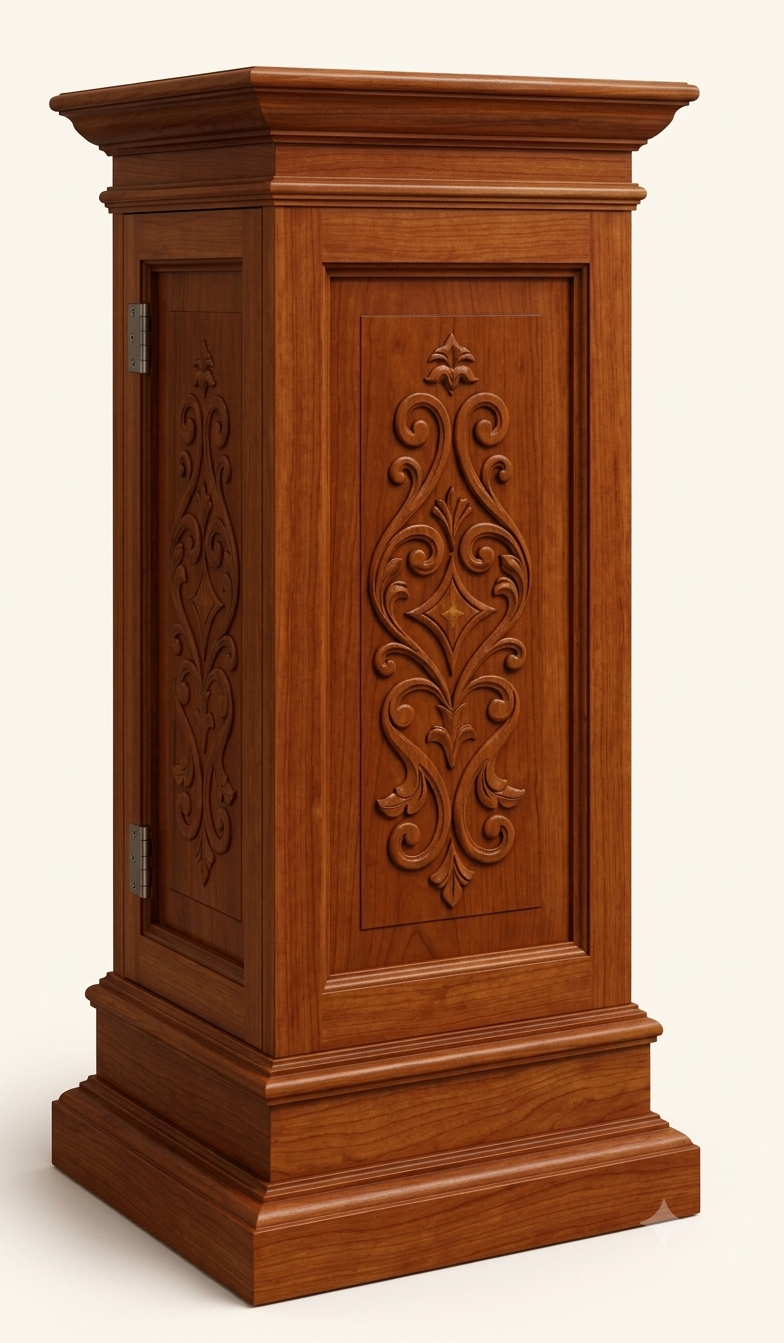
\includegraphics[width=0.35\textwidth]{../images/kego.png} 
\end{figure}
\end{minipage}
\hfill
\begin{minipage}[c]{0.45\textwidth}
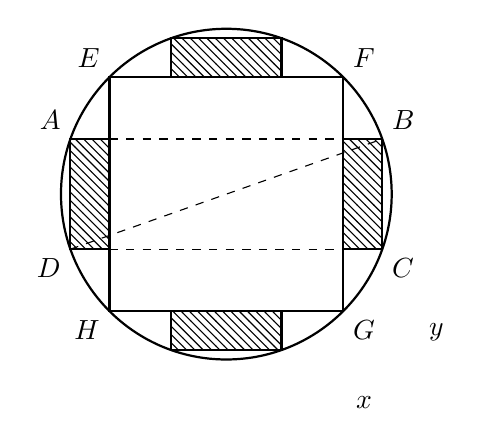
\begin{tikzpicture}[>=latex, scale=0.7]
    % Vẽ đường tròn
    \draw[thick] (0,0) circle (3cm);
    
    % Vẽ hình vuông EFGH nội tiếp
    \draw[thick] (2.121,-2.121) -- (2.121,2.121) -- (-2.121,2.121) -- (-2.121,-2.121) -- cycle;
    
    % Vẽ hình chữ nhật ABCD
    \draw[pattern=north west lines, pattern color=black, draw=black, thick] (-1,2.121) rectangle (1,2.83);
    \draw[pattern=north west lines, pattern color=black, draw=black, thick] (-1,-2.83) rectangle (1,-2.121);
    \draw[pattern=north west lines, pattern color=black, draw=black, thick] (-2.83,-1) rectangle (-2.121,1);
    \draw[pattern=north west lines, pattern color=black, draw=black, thick] (2.121,-1) rectangle (2.83,1);
    \draw[dashed] (-2.121,1) -- (2.121,1);
    \draw[dashed] (-2.121,-1) -- (2.121,-1); 
    \draw[dashed] (-2.83,-1) -- (2.83,1);
    % Đánh dấu các điểm
    \node[above left] at (-2.121,2.121) {$E$};
    \node[above right] at (2.121,2.121) {$F$};
    \node[below right] at (2.121,-2.121) {$G$};
    \node[below left] at (-2.121,-2.121) {$H$};
    \node[above left] at (-2.83,1) {$A$};
    \node[above right] at (2.83,1) {$B$};
    \node[below right] at (2.83,-1) {$C$};
    \node[below left] at (-2.83,-1) {$D$};
    
    % Nhãn x, y
    \node[below] at (2.5,-3.5) {$x$};
    \node[right] at (3.5,-2.5) {$y$};
\end{tikzpicture}
\end{minipage}
\end{center}

}{
    \textbf{a)} & Thiết diện ngang của trụ cột có độ dài cạnh là \( EF = 30\sqrt{2} \, (cm) \).
    & \textcolor{amberorange}{$\bigcirc$} & \textcolor{amberorange}{$\bigcirc$} \\ \hline
    
    \textbf{b)} & Hình chữ nhật \( ABCD \) có độ dài cạnh \( AB = 2x + 15\sqrt{2} \, (cm) \).
    & \textcolor{amberorange}{$\bigcirc$} & \textcolor{amberorange}{$\bigcirc$} \\ \hline
    
    \textbf{c)} & Ta có \( y = \sqrt{450 - 4x^2 - 60\sqrt{2}x} \, (cm) \).
    & \textcolor{amberorange}{$\bigcirc$} & \textcolor{amberorange}{$\bigcirc$} \\ \hline
    
    \textbf{d)} & Diện tích sử dụng theo thiết diện ngang lớn nhất của trụ cột cầu thang bằng \( 601 \, cm^2 \) (kết quả làm tròn đến hàng đơn vị).
    & \textcolor{amberorange}{$\bigcirc$} & \textcolor{amberorange}{$\bigcirc$} \\
}

% --- CÂU 4 ---
\questionTrueFalse{0}{4}{Bác thợ hàn dùng một thanh kim loại dài 300cm để uốn thành khung cửa sổ có dạng như hình vẽ. Gọi \( r \) là bán kính của nửa đường tròn.

\begin{center}
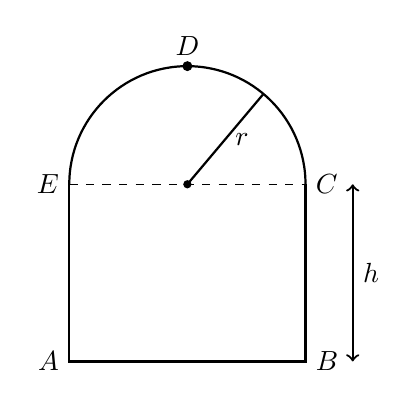
\begin{tikzpicture}[scale=1.5, thick]
        % Định nghĩa các điểm tọa độ gốc
        \coordinate (A) at (0,0);
        \coordinate (B) at (2,0);
        \coordinate (C) at (2,1.5);
        \coordinate (E) at (0,1.5);
        \coordinate (O) at (1,1.5); % Tâm của nửa đường tròn
        \coordinate (D) at (1,2.5); % Đỉnh cao nhất của nửa đường tròn

        % Vẽ khung hình chữ nhật phía dưới (khuyết cạnh trên)
        \draw (E) -- (A) -- (B) -- (C);

        % Vẽ nửa đường tròn phía trên từ điểm C đến E, tâm O, bán kính r = 1
        \draw (C) arc (0:180:1);

        % Vẽ đường đứt nét nối từ E sang C
        \draw[dashed, thin] (E) -- (C);

        % Vẽ tâm O (dấu chấm nhỏ)
        \fill (O) circle (1pt);

        % Vẽ điểm D (dấu chấm ở đỉnh đường tròn)
        \fill (D) circle (1.2pt) node[above] {$D$};

        % Vẽ bán kính r từ tâm O đến một điểm trên cung tròn (góc khoảng 50 độ)
        \draw (O) -- (1.64, 2.26) node[pos=0.5, right] {$r$};

        % Vẽ mũi tên kích thước chiều cao h bên phải
        \draw[<->] (2.4, 0) -- (2.4, 1.5) node[pos=0.5, right] {$h$};

        % Gán nhãn các đỉnh
        \node[left] at (A) {$A$};
        \node[right] at (B) {$B$};
        \node[right] at (C) {$C$};
        \node[left] at (E) {$E$};

    \end{tikzpicture}
\end{center}

}{
    \textbf{a)} & Diện tích của nửa hình tròn là \( S_1 = \dfrac{1}{2}\pi r^2 \, (cm^2) \).
    & \textcolor{amberorange}{$\bigcirc$} & \textcolor{amberorange}{$\bigcirc$} \\ \hline
    
    \textbf{b)} & Diện tích của hình chữ nhật là \( S_2 = 300r - \pi r^2 - 2r^2 \, (cm^2) \).
    & \textcolor{amberorange}{$\bigcirc$} & \textcolor{amberorange}{$\bigcirc$} \\ \hline
    
    \textbf{c)} & Khi \( r = 12 \) thì diện tích của khung cửa sổ nằm trong khoảng \( (2000; 3000) \) (đơn vị: \( cm^2 \)).
    & \textcolor{amberorange}{$\bigcirc$} & \textcolor{amberorange}{$\bigcirc$} \\ \hline
    
    \textbf{d)} & Biết \( r = r_0 \) thì diện tích của khung cửa sổ tạo thành đạt giá trị lớn nhất, khi đó \( r_0 \in (41; 42) \).
    & \textcolor{amberorange}{$\bigcirc$} & \textcolor{amberorange}{$\bigcirc$} \\
}

% --- CÂU 5 ---
\questionTrueFalse{0}{5}{Bác Nguyên muốn gò một cái thùng bằng tôn dạng hình hộp chữ nhật không nắp có đáy là hình vuông và đựng đầy được 256 lít nước. Gọi độ dài cạnh đáy của thùng là \( x \, (dm) \), chiều cao của thùng là \( h \, (dm) \).}{
    \textbf{a)} & Thể tích của thùng là \( V = x^2 h \, (dm^3) \).
    & \textcolor{amberorange}{$\bigcirc$} & \textcolor{amberorange}{$\bigcirc$} \\ \hline
    
    \textbf{b)} & Tổng diện tích xung quanh và diện tích đáy của thùng là  
    \(S(x) = x^2 + \dfrac{1024}{x} \, (dm^2).\)
    & \textcolor{amberorange}{$\bigcirc$} & \textcolor{amberorange}{$\bigcirc$} \\ \hline
    
    \textbf{c)} & Đạo hàm của hàm số \( S(x) \) là  
    \(S'(x) = 2x + \dfrac{1024}{x^2}.\)
    & \textcolor{amberorange}{$\bigcirc$} & \textcolor{amberorange}{$\bigcirc$} \\ \hline
    
    \textbf{d)} & Để gò được cái thùng mà tốn ít nguyên liệu nhất thì độ dài cạnh đáy của thùng là \( 7 \, (dm) \).
    & \textcolor{amberorange}{$\bigcirc$} & \textcolor{amberorange}{$\bigcirc$} \\
}

% --- CÂU 6 ---
\questionTrueFalse{0}{6}{Anh M chế tạo một bể cá có dạng khối hộp chữ nhật không nắp có thể tích 0,15 \( m^3 \), chiều cao \( h = 0,6m \), chiều rộng \( x \), chiều dài \( y \) (với \( x, y > 0 \)). Anh M dùng loại kính để làm các mặt bên có giá 60 000 đồng/\( m^2 \) và loại kính để làm đáy có giá 100 000 đồng/\( m^2 \)). Mọi chi phí khác xem như không đáng kể. Khi đó:}{
    \textbf{a)} & Biểu thức biểu diễn \( y \) theo \( x \) là \( y = \dfrac{0,25}{x} \).
    & \textcolor{amberorange}{$\bigcirc$} & \textcolor{amberorange}{$\bigcirc$} \\ \hline
    
    \textbf{b)} & Chi phí để làm các mặt xung quanh là  
    \(f(x) = 72000\left(x + \dfrac{0,25}{x}\right) \quad (\text{đơn vị: nghìn đồng}).\)
    & \textcolor{amberorange}{$\bigcirc$} & \textcolor{amberorange}{$\bigcirc$} \\ \hline
    
    \textbf{c)} & Với hàm số \( f(x) \) tìm được ở câu b, khi đó:  
    \(f'(x) = 0 \Leftrightarrow x = 0,5.\)
    & \textcolor{amberorange}{$\bigcirc$} & \textcolor{amberorange}{$\bigcirc$} \\ \hline
    
    \textbf{d)} & Chi phí thấp nhất để làm bể cá là 72 000 đồng.
    & \textcolor{amberorange}{$\bigcirc$} & \textcolor{amberorange}{$\bigcirc$} \\
}

% --- CÂU 7 ---
\questionTrueFalse{0}{7}{Một tấm kẽm hình vuông \( ABCD \) có cạnh bằng \( 30 \, \text{cm} \). Người ta gấp tấm kẽm theo hai cạnh \( EF \) và \( GH \) cho đến khi \( AD \) và \( BC \) trùng nhau như hình vẽ minh họa để được một hình lăng trụ khuyết hai đáy.

\begin{center}
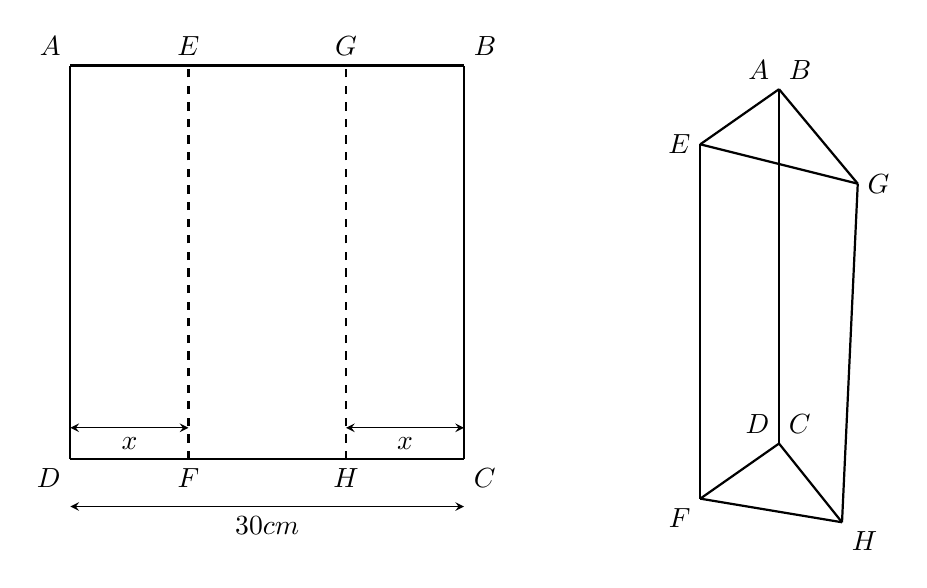
\begin{tikzpicture}[>=stealth]

    % Sơ đồ bên trái (Hình phẳng trước khi gấp)
    \begin{scope}[xshift=0cm]
        \draw[thick] (0,0) coordinate (D) -- (5,0) coordinate (C);
        \draw[thick] (C) -- (5,5) coordinate (B);
        \draw[thick] (B) -- (0,5) coordinate (A);
        \draw[thick] (A) -- (D);

        % Các đường nét đứt để gấp
        \draw[dashed, thick] (1.5,0) coordinate (F) -- (1.5,5) coordinate (E);
        \draw[dashed, thick] (3.5,0) coordinate (H) -- (3.5,5) coordinate (G);

        % Gán nhãn các điểm
        \node[above left] at (A) {$A$};
        \node[above right] at (B) {$B$};
        \node[below left] at (D) {$D$};
        \node[below right] at (C) {$C$};
        \node[above] at (E) {$E$};
        \node[below] at (F) {$F$};
        \node[above] at (G) {$G$};
        \node[below] at (H) {$H$};

        % Mũi tên kích thước và nhãn độ dài
        \draw[<->] (0,0.4) -- (1.5,0.4);
        \node[below] at (0.75,0.4) {$x$};
        
        \draw[<->] (3.5,0.4) -- (5,0.4);
        \node[below] at (4.25,0.4) {$x$};

        \draw[<->] (0,-0.6) -- (5,-0.6);
        \node[below] at (2.5,-0.6) {$30cm$};
    \end{scope}

    % Sơ đồ bên phải (Hình lăng trụ 3D sau khi gấp)
    \begin{scope}[xshift=8cm, yshift=-0.5cm]
        % Khởi tạo tọa độ theo góc nhìn phối cảnh giống hình gốc
        \coordinate (A3d) at (1.0, 5.2);
        \coordinate (B3d) at (1.0, 5.2);
        \coordinate (E3d) at (0.0, 4.5);
        \coordinate (G3d) at (2.0, 4.0);
        \coordinate (D3d) at (1.0, 0.7);
        \coordinate (C3d) at (1.0, 0.7);
        \coordinate (F3d) at (0.0, 0.0);
        \coordinate (H3d) at (1.8, -0.3);
        
        % Vẽ mặt đáy tam giác phía trên (EABG)
        \draw[thick] (E3d) -- (A3d);
        \draw[thick] (A3d) -- (B3d);
        \draw[thick] (B3d) -- (G3d);
        \draw[thick] (G3d) -- (E3d);

        % Vẽ mặt đáy tam giác phía dưới (FDHC)
        \draw[thick] (F3d) -- (D3d);
        \draw[thick] (D3d) -- (C3d);
        \draw[thick] (C3d) -- (H3d);
        \draw[thick] (H3d) -- (F3d);

        % Vẽ các cạnh đứng của hình lăng trụ
        \draw[thick] (E3d) -- (F3d);
        \draw[thick] (A3d) -- (D3d);
        \draw[thick] (B3d) -- (C3d);
        \draw[thick] (G3d) -- (H3d);
        
        % Gán nhãn các đỉnh phía trên
        \node[above left] at (A3d) {$A$};
        \node[above right] at (B3d) {$B$};
        \node[left] at (E3d) {$E$};
        \node[right] at (G3d) {$G$};

        % Gán nhãn các đỉnh phía dưới
        \node[above left] at (D3d) {$D$};
        \node[above right] at (C3d) {$C$};
        \node[below left] at (F3d) {$F$};
        \node[below right] at (H3d) {$H$};
    \end{scope}

\end{tikzpicture}
\end{center}

}{
    \textbf{a)} & Thể tích khối lăng trụ được tính bằng công thức \( V = 30S \, (cm^3) \), trong đó \( S \) là diện tích của tam giác \( AEG \).
    & \textcolor{amberorange}{$\bigcirc$} & \textcolor{amberorange}{$\bigcirc$} \\ \hline
    
    \textbf{b)} & Diện tích của tam giác \( AEG \) bằng  
    \( \sqrt{30} \sqrt{(15 - x)^2(2x - 15)} \, (cm^2) \).
    & \textcolor{amberorange}{$\bigcirc$} & \textcolor{amberorange}{$\bigcirc$} \\ \hline
    
    \textbf{c)} & Giá trị của \( x \) để thể tích khối lăng trụ lớn nhất là \( x = 10 \, (cm) \).
    & \textcolor{amberorange}{$\bigcirc$} & \textcolor{amberorange}{$\bigcirc$} \\ \hline
    
    \textbf{d)} & Thể tích khối lăng trụ lớn nhất bằng \( 1250 \, (cm^3) \).
    & \textcolor{amberorange}{$\bigcirc$} & \textcolor{amberorange}{$\bigcirc$} \\
}

% --- CÂU 8 ---
\questionTrueFalse{0}{8}{Nhân dịp ngày 1-6, bác T làm một cái đèn lồng cho con. Bác dùng một sợi dây đồng dài 12dm cắt thành 3 đoạn để uốn làm khung đèn. Đoạn thứ nhất bác uốn thành hình vuông \(ABCD\) có cạnh bằng \(x(dm)\) để làm đáy, hai đoạn còn lại có độ dài bằng nhau uốn thành các đường gấp khúc \(ASC\) và \(BSD\). Khung đèn sau khi hoàn thiện có hình dạng là một hình chóp tứ giác đều \(S.ABCD\) và mặt ngoài của đèn được dán giấy màu để trang trí (xem các mối nối, dán là không đáng kể).
\begin{center}

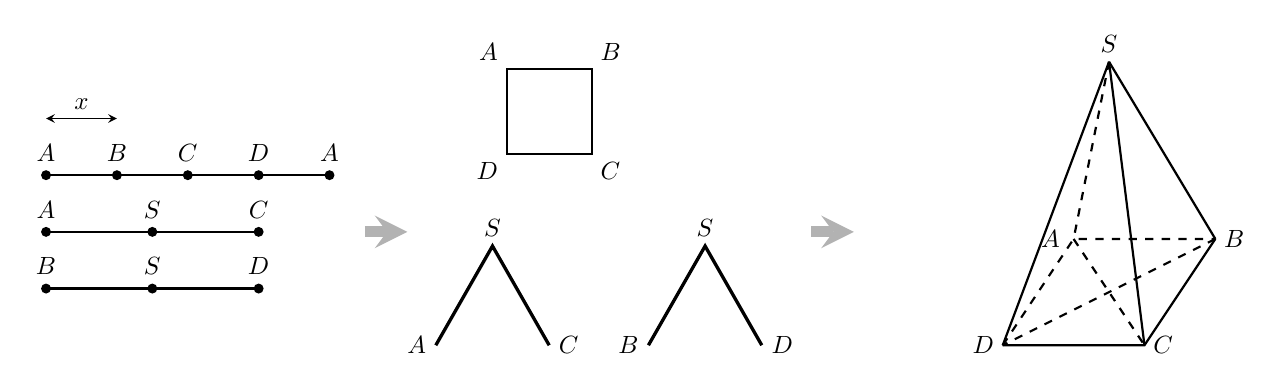
\begin{tikzpicture}[>=stealth, scale=0.9, every node/.style={transform shape}]

    % =================================================================
    % KHỐI 1: CÁC ĐOẠN THẲNG BÊN TRÁI
    % =================================================================
    \begin{scope}[xshift=0cm, yshift=0cm]
        % Thanh 1: A - B - C - D - A
        \draw[thick] (0,1.2) -- (4,1.2);
        \foreach \x/\txt in {0/A, 1/B, 2/C, 3/D, 4/A} {
            \fill (\x,1.2) circle (2pt);
            \node[above=2pt] at (\x,1.2) {$\txt$};
        }
        % Mũi tên x trên đoạn AB
        \draw[<->] (0,2) -- (1,2);
        \node[above] at (0.5,2) {$x$};

        % Thanh 2: A - S - C
        \draw[thick] (0,0.4) -- (3,0.4);
        \foreach \x/\txt in {0/A, 1.5/S, 3/C} {
            \fill (\x,0.4) circle (2pt);
            \node[above=2pt] at (\x,0.4) {$\txt$};
        }

        % Thanh 3: B - S - D
        \draw[thick] (0,-0.4) -- (3,-0.4);
        \foreach \x/\txt in {0/B, 1.5/S, 3/D} {
            \fill (\x,-0.4) circle (2pt);
            \node[above=2pt] at (\x,-0.4) {$\txt$};
        }
    \end{scope}

    % Mũi tên chuyển bước 1 -> 2
    \draw[->, line width=4pt, gray!60] (4.5,0.4) -- (5.1,0.4);

    % =================================================================
    % KHỐI 2: HÌNH VUÔNG VÀ CÁC CẶP ĐOẠN THẲNG Ở GIỮA
    % =================================================================
    \begin{scope}[xshift=6.5cm, yshift=0cm]
        % Hình vuông đáy ABCD ở trên
        \draw[thick] (0,1.5) rectangle (1.2,2.7);
        \node[above left] at (0,2.7) {$A$};
        \node[above right] at (1.2,2.7) {$B$};
        \node[below right] at (1.2,1.5) {$C$};
        \node[below left] at (0,1.5) {$D$};

        % Cặp chữ V bên trái: A - S - C
        \draw[very thick] (-1,-1.2) node[left] {$A$} -- (-0.2,0.2) node[above] {$S$} -- (0.6,-1.2) node[right] {$C$};
        
        % Cặp chữ V bên phải: B - S - D
        \draw[very thick] (2,-1.2) node[left] {$B$} -- (2.8,0.2) node[above] {$S$} -- (3.6,-1.2) node[right] {$D$};
    \end{scope}

    % Mũi tên chuyển bước 2 -> 3
    \draw[->, line width=4pt, gray!60] (10.8,0.4) -- (11.4,0.4);

    % =================================================================
    % KHỐI 3: HÌNH CHÓP S.ABCD 3D BÊN PHẢI
    % =================================================================
    \begin{scope}[xshift=13.5cm, yshift=-1.2cm]
        % Định nghĩa tọa độ các đỉnh hình chóp
        \coordinate (A) at (1,1.5);
        \coordinate (B) at (3,1.5);
        \coordinate (C) at (2,0);
        \coordinate (D) at (0,0);
        \coordinate (S) at (1.5,4);

        % Vẽ các cạnh khuất (nét đứt)
        \draw[dashed, thick] (D) -- (A) -- (B);
        \draw[dashed, thick] (A) -- (C);
        \draw[dashed, thick] (B) -- (D);
        \draw[dashed, thick] (S) -- (A);

        % Vẽ các cạnh nhìn thấy (nét liền)
        \draw[thick] (D) -- (C) -- (B);
        \draw[thick] (S) -- (D);
        \draw[thick] (S) -- (C);
        \draw[thick] (S) -- (B);

        % Gán nhãn các đỉnh
        \node[above] at (S) {$S$};
        \node[left=2pt] at (A) {$A$};
        \node[right] at (B) {$B$};
        \node[right] at (C) {$C$};
        \node[left] at (D) {$D$};
    \end{scope}

\end{tikzpicture}
\end{center}}
{
    \textbf{a)} & Độ dài cạnh bên của khung đèn bằng \(3 - x \, (dm)\).
    & \textcolor{amberorange}{$\bigcirc$} & \textcolor{amberorange}{$\bigcirc$} \\ \hline
    
    \textbf{b)} & Khi \(x = 1 \, (dm)\) thì độ dài đường cao của khung đèn là \(\sqrt{14} \, (dm)\).
    & \textcolor{amberorange}{$\bigcirc$} & \textcolor{amberorange}{$\bigcirc$} \\ \hline
    
    \textbf{c)} & Khi tất cả các cạnh bằng nhau thì diện tích giấy màu cần dùng là \(\dfrac{9}{4}(1 + \sqrt{3}) \, dm^2\).
    & \textcolor{amberorange}{$\bigcirc$} & \textcolor{amberorange}{$\bigcirc$} \\ \hline
    
    \textbf{d)} & Thể tích phần không gian của đèn lồng lớn nhất khi \(x = 1,3 \, dm\) (kết quả làm tròn đến hàng phần chục).
    & \textcolor{amberorange}{$\bigcirc$} & \textcolor{amberorange}{$\bigcirc$} \\
}

% --- CÂU 9 ---
\questionTrueFalse{0}{9}{Một tấm nhôm hình vuông cạnh 240 cm. Người ta cắt ở bốn góc của tấm nhôm đó bốn hình vuông bằng nhau, mỗi hình vuông có cạnh bằng \( x \) (cm), rồi gấp tấm nhôm lại như hình vẽ dưới đây để được một cái hộp không nắp.
\begin{center}
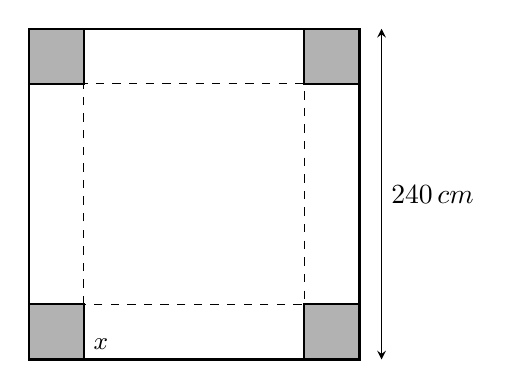
\begin{tikzpicture}[scale=0.35, >=stealth]
    % --- HÌNH 1: MẢNH CÁC TẤM BÌA PHẲNG ---
    % Khai báo kích thước tổng thể và cạnh cắt x
    \def\a{12}
    \def\x{2}
    
    % Tô màu xám cho 4 góc bị cắt
    \fill[gray!60] (0,0) rectangle (\x,\x);
    \fill[gray!60] (0,\a-\x) rectangle (\x,\a);
    \fill[gray!60] (\a-\x,0) rectangle (\a,\x);
    \fill[gray!60] (\a-\x,\a-\x) rectangle (\a,\a);
    \draw[thick] (0,0) rectangle (\x,\x);
    \draw[thick] (0,\a-\x) rectangle (\x,\a);
    \draw[thick] (\a-\x,0) rectangle (\a,\x);
    \draw[thick] (\a-\x,\a-\x) rectangle (\a,\a);
    % Vẽ biên ngoài hình vuông lớn
    \draw[thick] (0,0) rectangle (\a,\a);
    \draw[dashed] (\x,\x) rectangle (\a-\x,\a-\x);
   
    % Kí hiệu đoạn x ở góc
    \node at (\x, 0) [above right] {\small $x$};
    
    % Kí hiệu kích thước cạnh 12cm
    \draw[<->] (\a + 0.8, 0) -- (\a + 0.8, \a) node[midway, right] {$240\,cm$};
\end{tikzpicture}
\quad \quad \quad
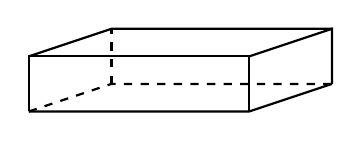
\begin{tikzpicture}[scale=0.35, >=stealth]
    % --- HÌNH 2: HÌNH HỘP CHỮ NHẬT 3D KHÔNG NẮP ---
    % Định nghĩa các điểm tọa độ mặt đáy
    \coordinate (A) at (0,0);
    \coordinate (B) at (8,0);
    \coordinate (C) at (11,1);
    \coordinate (D) at (3,1);
    
    % Chiều cao hộp h
    \def\h{2}
    
    % Các điểm mặt trên
    \coordinate (A1) at (0,\h);
    \coordinate (B1) at (8,\h);
    \coordinate (C1) at (11,3);
    \coordinate (D1) at (3,3);
    
    % Vẽ các nét khuất (nét đứt phía sau)
    \draw[dashed, thick] (A) -- (D) -- (C);
    \draw[dashed, thick] (D) -- (D1);
    
    % Vẽ các nét thấy phía trước và mặt trên mở
    \draw[thick] (A) -- (B) -- (C);
    \draw[thick] (A) -- (A1) -- (B1) -- (B);
    \draw[thick] (B1) -- (C1) -- (C);
    \draw[thick] (A1) -- (D1) -- (C1);
    
\end{tikzpicture}
\end{center}
}
{
    \textbf{a)} & Thể tích khối hộp nhận được khi tính theo \( x \) là  
    \(V = x(240 - 2x)^2.\)
    & \textcolor{amberorange}{$\bigcirc$} & \textcolor{amberorange}{$\bigcirc$} \\ \hline
    
    \textbf{b)} & Khi \( x = 20 \, cm \) thì thể tích của khối hộp nhận được là \( 8 \, m^3 \).
    & \textcolor{amberorange}{$\bigcirc$} & \textcolor{amberorange}{$\bigcirc$} \\ \hline
    
    \textbf{c)} & Để hộp nhận được có thể tích lớn nhất thì \( x = 60 \, cm \).
    & \textcolor{amberorange}{$\bigcirc$} & \textcolor{amberorange}{$\bigcirc$} \\ \hline
    
    \textbf{d)} & Hộp nhận được có thể tích lớn nhất là \( 1024 \, dm^3 \).
    & \textcolor{amberorange}{$\bigcirc$} & \textcolor{amberorange}{$\bigcirc$} \\
}

% --- CÂU 10 ---
\questionShortAnswer{0}{10}{Một chủ trang trại nuôi gia cầm muốn rào 2 chuồng hình chữ nhật sát nhau và sát một con sông, một chuồng nuôi gà và một chuồng nuôi vịt. Biết rằng chủ trang trại có 150m hàng rào và cạnh giáp với bờ sông thì không phải rào. Hỏi diện tích lớn nhất có thể bao quanh chuồng là bao nhiêu mét vuông?

\begin{center}
\begin{tikzpicture}[>=stealth, scale=0.9]

    % =================================================================
    % PHẦN 1: HÀNG RÀO LƯỚI B40 PHÍA TRÊN
    % =================================================================
    \begin{scope}[xshift=0cm, yshift=3.5cm]
        % Định nghĩa mẫu lưới (pattern) thủ công bằng vòng lặp để tạo lưới mắt cáo sắc nét
        % Khung lưới chữ nhật nền trắng ngăn các nét đè nhau
        \fill[white] (0,0) rectangle (9,1.5);
        
        % Các đường chéo xuôi
        \foreach \x in {-1.5,-1.2,...,9} {
            \draw[gray, thin] (\x,0) -- (\x+1.5,1.5);
        }
        % Các đường chéo ngược
        \foreach \x in {0.5,0.8,...,11} {
            \draw[gray, thin] (\x,0) -- (\x-1.5,1.5);
        }
        
        % Khung viền ngang của hàng rào
        \draw[thick, fill=gray!30] (0,-0.05) rectangle (9,0);
        \draw[thick, fill=gray!30] (0,1.5) rectangle (9,1.55);

        % Vẽ 3 cột trụ dọc (Trái, Giữa, Phải)
        \draw[thick, fill=gray!80] (-0.1,-0.1) rectangle (0.1,1.65);
        \draw[thick, fill=gray!80] (4.4,-0.1) rectangle (4.6,1.65);
        \draw[thick, fill=gray!80] (8.9,-0.1) rectangle (9.1,1.65);
        
        % Chốt bo đầu cột
        \draw[thick, fill=gray!90] (-0.15,1.65) rectangle (0.15,1.73);
        \draw[thick, fill=gray!90] (4.35,1.65) rectangle (4.65,1.73);
        \draw[thick, fill=gray!90] (8.85,1.65) rectangle (9.15,1.73);
    \end{scope}

    % =================================================================
    % PHẦN 2: BỜ SÔNG VÀ CHUỒNG GIA CẦM PHÍA DƯỚI
    % =================================================================
    \begin{scope}[xshift=0cm, yshift=0cm]
        % Dải màu xám đại diện cho Sông
        \draw[thick, fill=gray!70] (-0.2,1.2) rectangle (9.2,1.8);
        \node[above] at (4.5, 1.8) {\small Sông};

        % Khung chuồng gia cầm (Hình chữ nhật lớn ABCD có vách ngăn FE)
        \coordinate (A) at (1,1.2);
        \coordinate (B) at (1,0);
        \coordinate (C) at (8,0);
        \coordinate (D) at (8,1.2);
        \coordinate (E) at (6.3,0);
        \coordinate (F) at (6.3,1.2);

        % Vẽ các cạnh của chuồng (Nét liền đậm)
        \draw[thick] (A) -- (B) -- (C) -- (D);
        \draw[thick] (F) -- (E); % Vách ngăn bên trong

        % Điền chữ tên các đỉnh/điểm
        \node[below left] at (A) {$A$};
        \node[below left] at (B) {$B$};
        \node[below right] at (C) {$C$};
        \node[below right] at (D) {$D$};
        \node[below] at (E) {$E$};
        \node[below right] at (F) {$F$};

        % Ký hiệu biến x bên cạnh đoạn AB
        \node[left=3pt] at (1,0.4) {$x$};

        % Nhãn văn bản "Chuồng gia cầm" ở trung tâm lòng chuồng lớn
        \node at (3.6, 0.4) {\small Chuồng gia cầm};
    \end{scope}

\end{tikzpicture}
\end{center}}

% --- CÂU 11 ---
\questionShortAnswer{0}{11}{Một khuôn bánh cupcake được tạo nên từ hình vuông có cạnh bằng 8, người ta cắt bỏ các tam giác vuông cân để tạo thành hình tô đậm như hình vẽ. Sau đó người ta gập thành hình hộp chữ nhật không nắp rồi đổ bột bánh vào. Thể tích lớn nhất của khuôn bánh bằng bao nhiêu (kết quả làm tròn đến hàng phần mười)?

\begin{center}
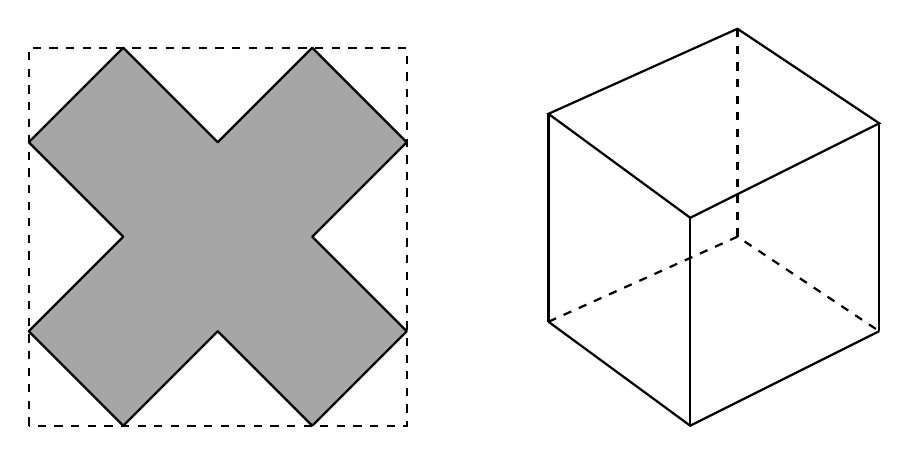
\begin{tikzpicture}[>=stealth, scale=1.2]

    % =================================================================
    % HÌNH BÊN TRÁI: HÌNH CHỮ THẬP TRONG KHUNG VUÔNG NÉT ĐỨT
    % =================================================================
    \begin{scope}[xshift=0cm, yshift=0cm]
        % Vẽ khung hình vuông nét đứt
        \draw[dashed, thick] (0,0) rectangle (4,4);

        % Vẽ và tô màu xám cho hình chữ thập (cross)
        \draw[thick, fill=gray!70, line join=round] 
            (0,3) -- (1,4) -- (2,3) -- (3,4) -- (4,3) -- (3,2) 
            -- (4,1) -- (3,0) -- (2,1) -- (1,0) -- (0,1) -- (1,2) -- cycle;
    \end{scope}

    % =================================================================
    % HÌNH BÊN PHẢI: HÌNH LẬP PHƯƠNG KHÔNG GIAN (3D)
    % =================================================================
    \begin{scope}[xshift=5.5cm, yshift=0cm]
        % Định nghĩa tọa độ các đỉnh của hình lập phương
        % Các đỉnh mặt đáy
        \coordinate (A) at (2,2); % Đỉnh khuất phía sau
        \coordinate (B) at (0,1.1);   % Đỉnh bên trái
        \coordinate (C) at (1.5,0);   % Đỉnh thấp nhất phía trước
        \coordinate (D) at (3.5,1);   % Đỉnh bên phải

        % Các đỉnh mặt trên
        \coordinate (A1) at (2,4.2);
        \coordinate (B1) at (0,3.3);
        \coordinate (C1) at (1.5,2.2);
        \coordinate (D1) at (3.5,3.2);

        % Vẽ các cạnh khuất (nét đứt) gắn với đỉnh A
        \draw[dashed, thick] (B) -- (A) -- (D);
        \draw[dashed, thick] (A) -- (A1);

        % Vẽ các cạnh nhìn thấy của mặt đáy và các cạnh bên (nét liền)
        \draw[thick] (B) -- (C) -- (D);
        \draw[thick] (B) -- (B1);
        \draw[thick] (C) -- (C1);
        \draw[thick] (D) -- (D1);

        % Vẽ các cạnh của mặt trên (nét liền)
        \draw[thick] (A1) -- (B1) -- (C1) -- (D1) -- cycle;
    \end{scope}

\end{tikzpicture}
\end{center}}

% --- CÂU 12 ---
\questionShortAnswer{0}{12}{Người ta muốn thiết kế một bể cá bằng kính không có nắp với thể tích \( 162 \, dm^3 \), chiều cao là \( 3 \, dm \). Một vách ngăn (cùng bằng kính) ở giữa, chia bể cá thành hai ngăn, với các kích thước \( a, b \, (dm) \) như hình vẽ. Biết rằng khi \( a = a_0; b = b_0 \) thì việc làm kính cho bể cá tốn ít nguyên liệu nhất. Tính giá trị của \( T = a_0 + 2b_0 \).

\begin{center}
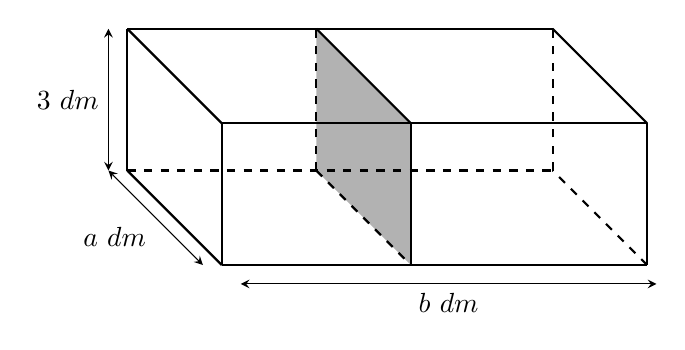
\begin{tikzpicture}[>=stealth, scale=1.2]

    % =================================================================
    % ĐỊNH NGHĨA CÁC TỌA ĐỘ ĐỈNH (HÌNH HỘP CHỮ NHẬT)
    % =================================================================
    % Các đỉnh mặt đáy phía sau
    \coordinate (A) at (0,1);
    \coordinate (A_mid) at (2,1);
    \coordinate (A_end) at (4.5,1);

    % Các đỉnh mặt đáy phía trước
    \coordinate (B) at (1,0);
    \coordinate (B_mid) at (3,0);
    \coordinate (B_end) at (5.5,0);

    % Các đỉnh mặt trên phía sau
    \coordinate (C) at (0,2.5);
    \coordinate (C_mid) at (2,2.5);
    \coordinate (C_end) at (4.5,2.5);

    % Các đỉnh mặt trên phía trước
    \coordinate (D) at (1,1.5);
    \coordinate (D_mid) at (3,1.5);
    \coordinate (D_end) at (5.5,1.5);

    % =================================================================
    % VẼ VÀ TÔ MÀU MẶT CẮT Ở GIỮA
    % =================================================================
    \fill[gray!60] (A_mid) -- (B_mid) -- (D_mid) -- (C_mid) -- cycle;

    % =================================================================
    % VẼ CÁC CẠNH KHUẤT (NÉT ĐỨT)
    % =================================================================
    \draw[dashed, thick] (A) -- (A_end);
    \draw[ thick] (A) -- (B);
    \draw[ thick] (A) -- (C);
    \draw[dashed, thick] (A_end) -- (C_end);
    \draw[dashed, thick] (A_mid) -- (C_mid);
    \draw[dashed, thick] (A_mid) -- (B_mid);

    % =================================================================
    % VẼ CÁC CẠNH NHÌN THẤY (NÉT LIỀN)
    % =================================================================
    % Mặt đáy phía trước
    \draw[thick] (B) -- (B_end);
    \draw[dashed,thick] (B_end) -- (A_end);
    
    % Các cạnh đứng phía trước
    \draw[thick] (B) -- (D);
    \draw[thick] (B_mid) -- (D_mid);
    \draw[thick] (B_end) -- (D_end);

    % Mặt phía trên
    \draw[thick] (C) -- (C_end);
    \draw[thick] (D) -- (D_end);
    \draw[thick] (C) -- (D);
    \draw[thick] (C_mid) -- (D_mid);
    \draw[thick] (C_end) -- (D_end);

    % =================================================================
    % VẼ CÁC MŨI TÊN KÍCH THƯỚC VÀ ĐIỀN THÔNG SỐ
    % =================================================================
    % Chiều cao 3 dm (bên trái)
    \draw[<->] (-0.2,1) -- (-0.2,2.5);
    \node[left] at (-0.2,1.75) {$3\ dm$};

    % Chiều rộng a dm (cạnh đáy bên trái)
    \draw[<->] (-0.2,1) -- (0.8,0);
    \node[below left] at (0.3,0.5) {$a\ dm$};

    % Chiều dài b dm (cạnh đáy phía trước)
    \draw[<->] (1.2,-0.2) -- (5.6,-0.2);
    \node[below] at (3.4,-0.2) {$b\ dm$};

\end{tikzpicture}
\end{center}}

% --- CÂU 13 ---
\questionShortAnswer{0}{13}{Anh Tú dự định làm một cái thùng đựng nước hình trụ bằng nhôm có nắp đậy có thể tích \( 30 \, m^3 \). Chi phí làm mỗi \( m^2 \) đáy là 200 000 đồng, mỗi \( m^2 \) nắp là 100 000 đồng và mỗi \( m^2 \) mặt xung quanh là 150 000 đồng. Để chi phí làm thùng là thấp nhất thì anh Tú nên làm chiếc thùng với chiều cao là bao nhiêu mét? (Xem độ dài của tấm nhôm là không đáng kể, kết quả làm tròn đến hàng phần trăm).}

% --- CÂU 14 ---
\questionShortAnswer{0}{14}{Cho một tấm tôn hình tròn có diện tích \( 8\pi \, dm^2 \). Người ta cắt thành một hình quạt có góc ở tâm là \( \alpha \, (0 < \alpha < 2\pi) \) như Hình 1 để làm thành một cái gầu múc nước hình nón như ở Hình 2. Hỏi thể tích lớn nhất của cái gầu là bao nhiêu lít (kết quả làm tròn đến hàng phần trăm)?

\begin{center}
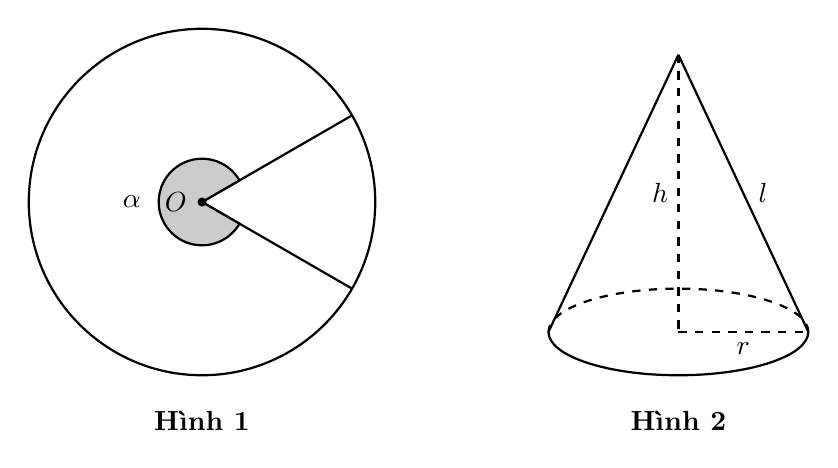
\begin{tikzpicture}[>=stealth, scale=1.1]

    % =================================================================
    % HÌNH 1: HÌNH QUẠT TRÒN BÊN TRÁI
    % =================================================================
    \begin{scope}[xshift=0cm, yshift=0cm]
        \coordinate (O) at (0,0);
        
        % Vẽ đường tròn lớn
        \draw[thick] (O) circle (2);
        
        % Vẽ 2 bán kính giới hạn hình quạt (ví dụ góc 30 độ và 330 độ)
        \draw[thick] (O) -- (30:2);
        \draw[thick] (O) -- (-30:2);
        
        % Vẽ phần quạt tròn nhỏ được tô màu xám biểu diễn góc alpha
        \fill[gray!40, draw=black, thick] (O) -- (30:0.5) arc (30:330:0.5) -- cycle;
        
        % Tâm O
        \fill (O) circle (1.5pt) node[left=2pt] {$O$};
        
        % Ký hiệu góc alpha
        \node[left=3pt] at (180:0.5) {$\alpha$};
        
        % Nhãn Hình 1
        \node[below] at (0,-2.3) {\textbf{Hình 1}};
    \end{scope}

    % =================================================================
    % HÌNH 2: HÌNH NÓN 3D BÊN PHẢI
    % =================================================================
    \begin{scope}[xshift=5.5cm, yshift=-0.5cm]
        \coordinate (I) at (0,-1);       % Tâm đường tròn đáy
        \coordinate (S) at (0,2.2);     % Đỉnh hình nón
        \coordinate (A) at (-1.5,-1);    % Điểm ngoài cùng bên trái đáy
        \coordinate (B) at (1.5,-1);     % Điểm ngoài cùng bên phải đáy

        % Vẽ nửa elip phía trước đáy (nét liền)
        \draw[thick] (A) arc (180:360:1.5 and 0.5);
        
        % Vẽ nửa elip phía sau đáy (nét đứt)
        \draw[dashed, thick] (B) arc (0:180:1.5 and 0.5);
        
        % Vẽ 2 đường sinh bên ngoài (nét liền)
        \draw[thick] (S) -- (A);
        \draw[thick] (S) -- (B);
        
        % Vẽ chiều cao h và bán kính r bên trong nón (nét đứt)
        \draw[dashed, thick] (S) -- (I) node[pos=0.5, left] {$h$};
        \draw[dashed, thick] (I) -- (B) node[pos=0.5, below] {$r$};
        
        % Ký hiệu đường sinh l
        \node[right=2pt] at (0.75, 0.6) {$l$};
        
        % Nhãn Hình 2
        \node[below] at (0,-1.8) {\textbf{Hình 2}};
    \end{scope}

\end{tikzpicture}
\end{center}}

% --- CÂU 15 ---
\questionShortAnswer{0}{15}{Một thùng chứa nhiên liệu gồm phần ở giữa là một hình trụ có chiều dài \( h \, (m) \) và hai đầu là các nửa hình cầu bán kính \( r \, (m) \) (hình vẽ). Biết rằng thể tích của thùng chứa là \( 288\,000\pi \, (m^3) \). Để sơn mặt ngoài của phần hình cầu cần 20 000 đồng trên \( 1m^2 \), còn sơn mặt ngoài cho phần hình trụ cần 10 000 đồng trên \( 1m^2 \). Để chi phí cho việc sơn diện tích mặt ngoài thùng chứa (bao gồm diện tích xung quanh của hình trụ và diện tích hai nửa hình cầu) là nhỏ nhất thì \( r \) bằng bao nhiêu mét (biết rằng bán kính \( r \) không vượt quá \( 50 \, m \), kết quả làm tròn đến hàng đơn vị)?

\begin{center}
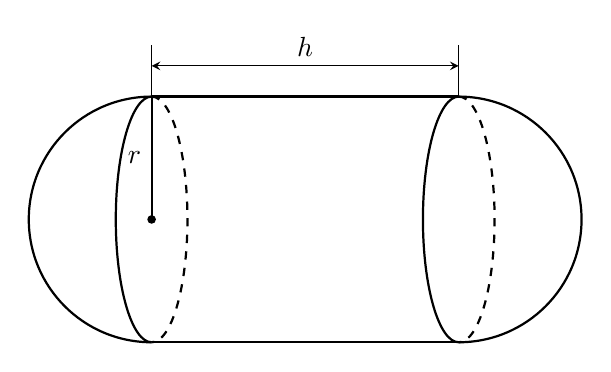
\begin{tikzpicture}[>=stealth, scale=1.3]

    % =================================================================
    % 1. ĐỊNH NGHĨA THÔNG SỐ VÀ TỌA ĐỘ CƠ BẢN
    % =================================================================
    \def\r{1.2}    % Bán kính đáy/bán cầu
    \def\h{3.0}    % Chiều dài phần hình trụ
    
    \coordinate (O1) at (0,0);      % Tâm đáy bên trái
    \coordinate (O2) at (\h,0);     % Tâm đáy bên phải

    % =================================================================
    % 2. VẼ PHẦN KHUẤT (NẾT ĐỨT) PHÍA SAU
    % =================================================================
    % Nửa elip phía sau của đáy trái và đáy phải
    \draw[dashed, thick] (O1) ++(0,\r) arc (90:-90:0.35 and \r);
    \draw[dashed, thick] (O2) ++(0,\r) arc (90:-90:0.35 and \r);

    % =================================================================
    % 3. VẼ PHẦN NHÌN THẤY (NÉT LIỀN)
    % =================================================================
    % Nửa elip phía trước của đáy trái và đáy phải
    \draw[thick] (O1) ++(0,\r) arc (90:270:0.35 and \r);
    \draw[thick] (O2) ++(0,\r) arc (90:270:0.35 and \r);

    % Hai đường sinh nối phần hình trụ (trên và dưới)
    \draw[thick] (0,\r) -- (\h,\r);
    \draw[thick] (0,-\r) -- (\h,-\r);

    % Hai vòm bán cầu ở hai đầu (Trái và Phải)
    \draw[thick] (0,\r) arc (90:270:\r);
    \draw[thick] (\h,\r) arc (90:-90:\r);

    % =================================================================
    % 4. VẼ BÁN KÍNH R VÀ THÔNG SỐ H
    % =================================================================
    % Tâm và bán kính r ở đáy trái
    \fill (O1) circle (1.2pt);
    \draw[thick] (O1) -- (0,\r) node[pos=0.5, left=0.1pt] {$r$};

    % Mũi tên kích thước biểu diễn chiều dài h phía trên
    \draw[<->] (0, \r + 0.3) -- (\h, \r + 0.3) node[pos=0.5, above] {$h$};
    
    % Các đường giới hạn nhỏ cho mũi tên h
    \draw[thin] (0, \r) -- (0, \r + 0.5);
    \draw[thin] (\h, \r) -- (\h, \r + 0.5);

\end{tikzpicture}
\end{center}}

% --- CÂU 16 ---
\questionShortAnswer{0}{16}{Ông \( B \) dự định sử dụng hết \( 6 \, m^2 \) kính để làm một bể cá bằng kính có dạng hình hộp chữ nhật không nắp, chiều dài gấp đôi chiều rộng (các mối ghép có kích thước không đáng kể). Hỏi ông \( B \) có thể làm được bể cá có dung tích lớn nhất bằng bao nhiêu \( m^3 \) (kết quả làm tròn đến hàng phần trăm)?}

% --- CÂU 17 ---
\questionShortAnswer{0}{17}{Một nhóm bạn đi picnic muốn cắm trại qua đêm. Biết trại cắm là một hình chóp đỉnh \( S \) cách đều các chân trại \( A, B, C \) một đoạn bằng \( 4m \). Biết đáy trại là một tam giác vuông tại \( A \) và \( AB = 2m \). Nhóm muốn cắm trại sao cho thể tích của trại là lớn nhất cho không gian thoải mái. Khi đó độ dài \( AC \) bằng bao nhiêu mét (kết quả làm tròn đến hàng phần trăm)?}

% --- CÂU 18 ---
\questionShortAnswer{0}{18}{Ông Dương muốn làm một cái phễu hình nón có thể tích bằng \( 9\pi\sqrt{2} \). Ông Dương muốn dùng tôn để làm phần mặt xung quanh của phễu. Hỏi bán kính đáy của cái phễu bằng bao nhiêu để diện tích tôn mà ông Dương cần dùng là nhỏ nhất?}

% --- CÂU 19 ---
\questionShortAnswer{0}{19}{Để chặn đường hành lang hình chữ \( L \), người ta dùng một que sào thẳng dài đặt kín những điểm chạm với hành lang (như hình vẽ). Biết \( a = 18 \) và \( b = 2 \), hỏi cái sào thỏa mãn điều kiện trên có chiều dài ngắn nhất là bao nhiêu (kết quả làm tròn đến hàng phần mười).

\begin{center}
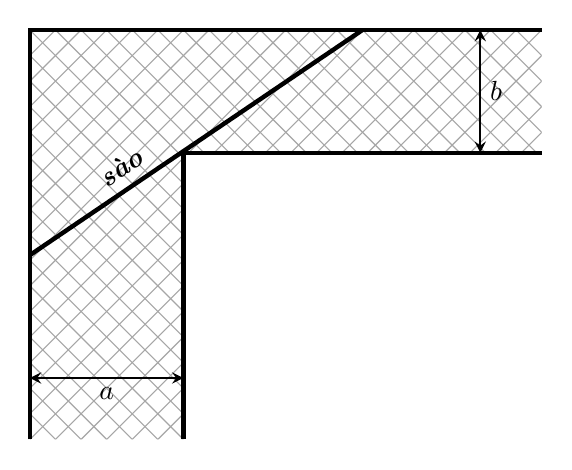
\begin{tikzpicture}[>=stealth, scale=1.3]

    % =================================================================
    % 1. VẼ VÀ TÔ MẪU LƯỚI GẠCH GÓC HÀNH LANG (L-SHAPE)
    % =================================================================
    \begin{scope}
        % Định nghĩa vùng bao hình chữ L để giới hạn vùng gạch kẻ
        \clip (0,0) -- (0,4) -- (5,4) -- (5,2.8) -- (1.5,2.8) -- (1.5,0) -- cycle;
        
        % Tô nền trắng để chống đè nét
        \fill[white] (0,0) rectangle (5,4);
        
        % Tạo mẫu lưới gạch đan chéo (gần giống hình gốc)
        \foreach \x in {-4,-3.75,...,5} {
            \draw[gray!70, thin] (\x,0) -- (\x+4,4);
        }
        \foreach \x in {0,0.25,...,9} {
            \draw[gray!70, thin] (\x,0) -- (\x-4,4);
        }
    \end{scope}

    % =================================================================
    % 2. VẼ CÁC ĐƯỜNG BIÊN HÀNH LANG
    % =================================================================
    % Biên ngoài cùng bên trái và phía trên
    \draw[ultra thick] (0,0) -- (0,4) -- (5,4);
    
    % Góc tường phía trong
    \draw[ultra thick] (1.5,0) -- (1.5,2.8) -- (5,2.8);

    % =================================================================
    % 3. VẼ THANH SÀO CHẮN GÓC (ĐOẠN THẲNG NGHIÊNG)
    % =================================================================
    % Tọa độ thanh sào đi qua góc tường (1.5, 2.8)
    \coordinate (P1) at (0, 1.8);
    \coordinate (P2) at (3.25, 4);
    \draw[ultra thick, black] (P1) -- (P2);
    
    % Nhãn chữ "sào" xoay nghiêng dọc theo thanh sào
    \node[above=2pt, rotate=34] at (1.0, 2.45) {\textbf{\textit{sào}}};

    % =================================================================
    % 4. VẼ KÍCH THƯỚC A VÀ B VỚI MŨI TÊN HAI ĐẦU
    % =================================================================
    % Kích thước chiều rộng hành lang đứng 'a'
    \draw[<->, thick] (0,0.6) -- (1.5,0.6);
    \node[below] at (0.75,0.6) {$a$};

    % Kích thước chiều rộng hành lang ngang 'b'
    \draw[<->, thick] (4.4,2.8) -- (4.4,4);
    \node[right] at (4.4,3.4) {$b$};

\end{tikzpicture}
\end{center}}

% --- CÂU 20 ---
\questionShortAnswer{0}{20}{Cho một tấm bìa hình chữ nhật có chiều dài \( AB = 80 \, \text{cm} \), chiều rộng \( BC = 60 \, \text{cm} \). Người ta cắt 6 hình vuông bằng nhau như hình vẽ, mỗi hình vuông cạnh bằng \( x \, \text{cm} \), rồi gập tấm bìa lại như hình vẽ để được một hộp quà có nắp. Tìm \( x \) để hộp nhận được có thể tích lớn nhất (kết quả làm tròn đến hàng phần mười)?

\begin{center}
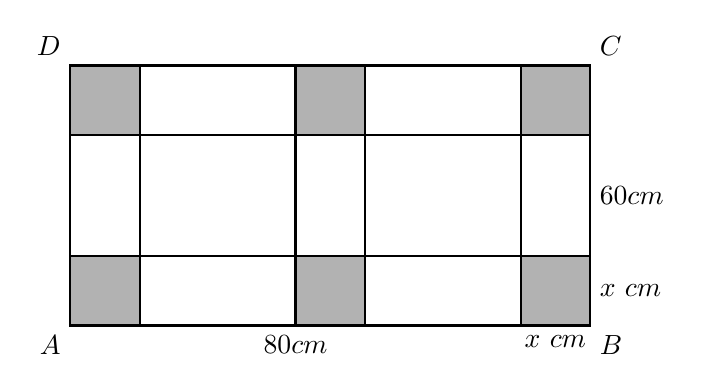
\begin{tikzpicture}[>=stealth, scale=1.1]

    % =================================================================
    % 1. ĐỊNH NGHĨA KÍCH THƯỚC VÀ TÔ MÀU CÁC HÌNH VUÔNG XÁM Ở GÓC VÀ GIỮA
    % =================================================================
    % Kích thước tổng thể hình chữ nhật ABCD: rộng 6 units (80cm), cao 3 units (60cm)
    % Cạnh hình vuông nhỏ x là 0.8 units
    \def\x{0.8}
    \def\w{6.0}
    \def\h{3.0}
    \def\mid{3.0} % Vị trí tâm dải ở giữa

    % Tô màu xám cho các hình vuông nhỏ
    \fill[gray!60] (0,0) rectangle (\x,\x);
    \fill[gray!60] (0,\h-\x) rectangle (\x,\h);
    \fill[gray!60] (\w-\x,0) rectangle (\w,\x);
    \fill[gray!60] (\w-\x,\h-\x) rectangle (\w,\h);
    
    % Hai ô ở chính giữa cạnh trên và cạnh dưới
    \fill[gray!60] (\mid-\x/2,0) rectangle (\mid+\x/2,\x);
    \fill[gray!60] (\mid-\x/2,\h-\x) rectangle (\mid+\x/2,\h);

    % =================================================================
    % 2. VẼ KHUNG VÀ CÁC ĐƯỜNG PHÂN CHIA NẾT LIỀN
    % =================================================================
    % Khung hình chữ nhật lớn ngoài cùng ABCD
    \draw[thick] (0,0) rectangle (\w,\h);

    % Các đường kẻ dọc phân chia
    \draw[thick] (\x,0) -- (\x,\h);
    \draw[thick] (\mid-\x/2,0) -- (\mid-\x/2,\h);
    \draw[thick] (\mid+\x/2,0) -- (\mid+\x/2,\h);
    \draw[thick] (\w-\x,0) -- (\w-\x,\h);

    % Các đường kẻ ngang phân chia
    \draw[thick] (0,\x) -- (\w,\x);
    \draw[thick] (0,\h-\x) -- (\w,\h-\x);

    % =================================================================
    % 3. GÁN NHÃN CÁC ĐỈNH VÀ THÔNG SỐ KÍCH THƯỚC
    % =================================================================
    % Tên bốn đỉnh chính
    \node[below left] at (0,0) {$A$};
    \node[below right] at (\w,0) {$B$};
    \node[above right] at (\w,\h) {$C$};
    \node[above left] at (0,\h) {$D$};

    % Các thông số kích thước bằng chữ (text)
    \node[below] at (\w/2-\x/2,0) {$80cm$};
    \node[below] at (\w-\x/2,0) {$x\ cm$};
    
    \node[right] at (\w,\x/2) {$x\ cm$};
    \node[right] at (\w,\h/2) {$60cm$};

\end{tikzpicture}
\end{center}}

% --- CÂU 21 ---
\questionShortAnswer{0}{21}{Một mảnh giấy hình chữ nhật có chiều dài 18cm và chiều rộng 9cm. Thực hiện thao tác gấp góc dưới bên phải sao cho đỉnh được gấp nằm trên cạnh chiều dài còn lại (như hình vẽ). Hỏi chiều dài \( L \) tối thiểu của nếp gấp là bao nhiêu \( cm \) (kết quả làm tròn đến hàng phần mười)?

\begin{center}
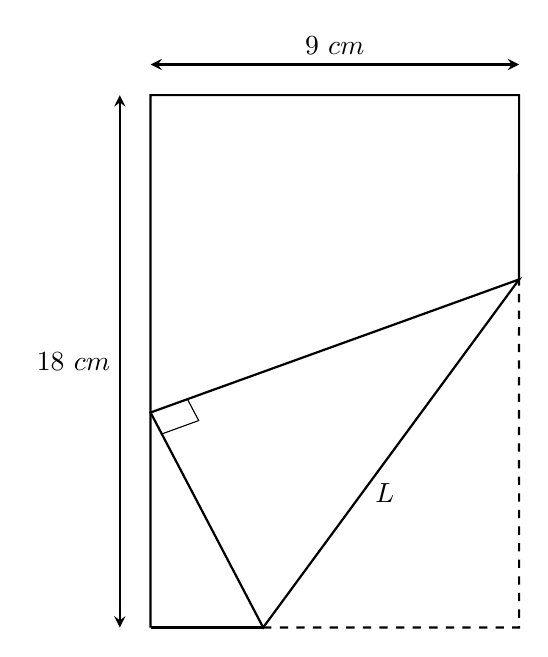
\begin{tikzpicture}[>=stealth, scale=1.3]

    % =================================================================
    % 1. ĐỊNH NGHĨA TỌA ĐỘ CÁC ĐIỂM CHÍNH (Hình chữ nhật 3.6 x 5.2 units)
    % =================================================================
    \coordinate (BottomLeft) at (0,0);
    \coordinate (TopLeft) at (0,5.2);
    \coordinate (TopRight) at (3.6,5.2);
    \coordinate (BottomRight) at (3.6,0);
    
    % Các điểm của tam giác gấp
    \coordinate (FoldBottom) at (1.1,0);
    \coordinate (FoldLeft) at (0,2.1);
    \coordinate (FoldRight) at (3.6,3.4);

    % =================================================================
    % 2. VẼ CÁC ĐƯỜNG BIÊN VÀ NÉT ĐỨT PHÂN CHIA
    % =================================================================
    % Vẽ các cạnh liền của khung hình chữ nhật
    \draw[thick] (BottomLeft) -- (TopLeft) -- (TopRight) -- (3.6, 3.4);
    \draw[thick] (BottomLeft) -- (FoldBottom);

    % Vẽ các cạnh nét đứt (phần giấy bị gấp hoặc khuất)
    \draw[dashed, thick] (FoldBottom) -- (BottomRight) -- (3.6, 3.4);

    % Vẽ tam giác gấp nội tiếp (Nét liền đậm)
    \draw[thick] (FoldBottom) -- (FoldLeft) -- (FoldRight) -- cycle;

    % =================================================================
    % 3. VẼ KÝ HIỆU GÓC VUÔNG VÀ ĐIỀN NHÃN L
    % =================================================================
    % Ký hiệu góc vuông tại vị trí FoldLeft (0, 2.1)
    \coordinate (P_B) at ($(FoldLeft)!0.1!(FoldBottom)$);
    \coordinate (P_C) at ($(FoldLeft)!0.1!(FoldRight)$);
    \coordinate (P_Corner) at ($(P_B) + (P_C) - (FoldLeft)$);
    \draw[thin] (P_B) -- (P_Corner) -- (P_C);
    % Nhãn chữ L đại diện cho chiều dài nếp gấp
    \node[below right] at (2.1, 1.5) {$L$};

    % =================================================================
    % 4. VẼ MŨI TÊN KÍCH THƯỚC CHIỀU RỘNG VÀ CHIỀU CAO
    % =================================================================
    % Chiều rộng 9 cm phía trên
    \draw[<->, thick] (0, 5.5) -- (3.6, 5.5);
    \node[above] at (1.8, 5.5) {$9\ cm$};

    % Chiều cao 18 cm phía bên trái
    \draw[<->, thick] (-0.3, 0) -- (-0.3, 5.2);
    \node[left] at (-0.3, 2.6) {$18\ cm$};

\end{tikzpicture}
\end{center}}

% --- CÂU 22 ---
\questionShortAnswer{0}{22}{Hình dưới đây là mương dẫn nước thủy lợi tại một địa phương phục vụ tưới tiêu cho ruộng đồng. Phần không gian trong mương để nước chảy có mặt cắt ngang là hình chữ nhật \(ABCD\). Với điều kiện lưu lượng nước qua mương cho phép thì diện tích mặt cắt \(ABCD\) là \(0,48 \, m^2\). Để đảm bảo yêu cầu kỹ thuật tốt nhất cho mương, người ta cần thiết kế sao cho tổng độ dài \(T = AB + BC + CD\) là ngắn nhất. Khi đó chiều rộng đáy mương bằng bao nhiêu mét (biết chiều rộng phải dưới \(1 \, m\), kết quả làm tròn đến hàng phần trăm)?

\begin{center}
\begin{tikzpicture}[>=stealth, scale=1.1]

    % =================================================================
    % HÌNH BÊN TRÁI: CHÈN FILE ẢNH PNG CỦA BẠN
    % =================================================================
    \begin{scope}[xshift=0cm, yshift=0cm]
        \node[anchor=south west, inner sep=0] at (0,0) {
            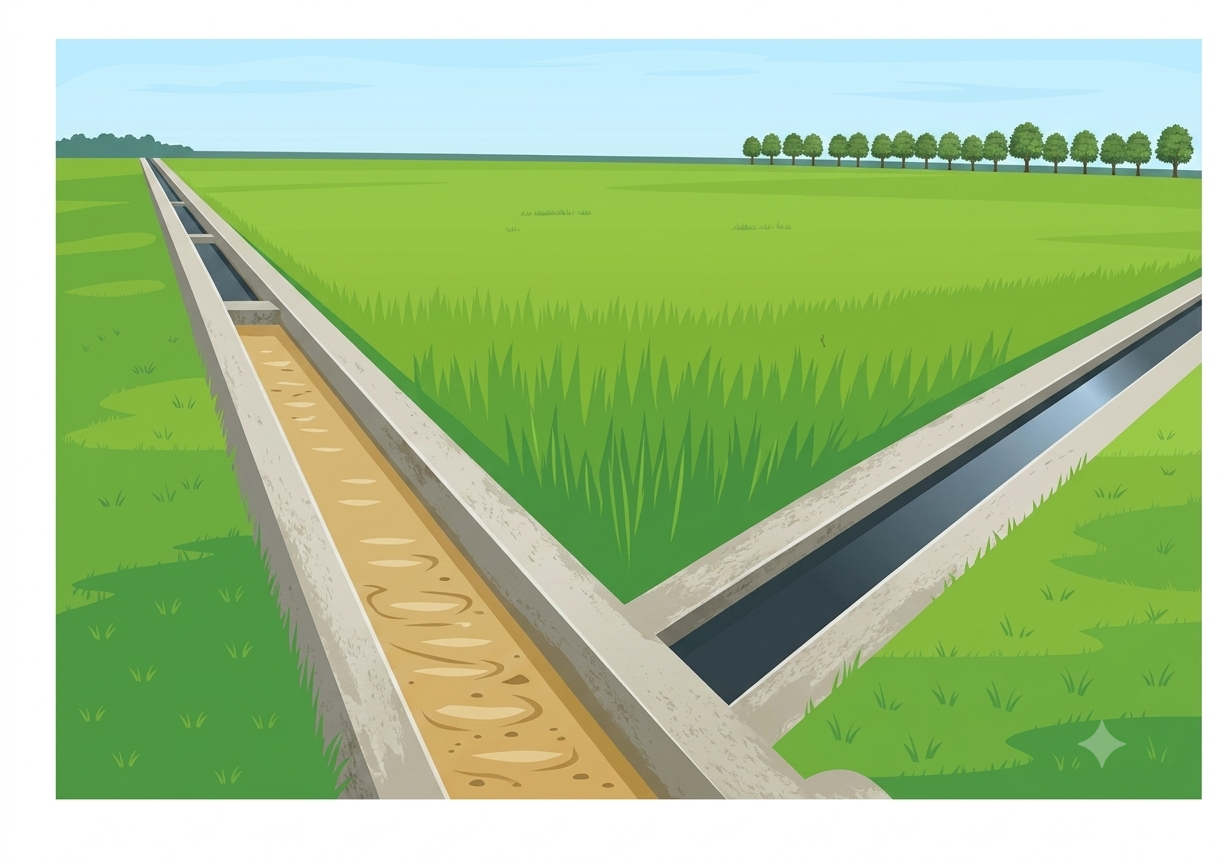
\includegraphics[width=5cm]{../images/MuongRuong.png}
        };
    \end{scope}

    % =================================================================
    % HÌNH BÊN PHẢI: MẶT CẮT NGANG CỦA MƯƠNG (HÌNH CHỮ U)
    % =================================================================
    \begin{scope}[xshift=6.0cm, yshift=0.2cm]
        
        % Vẽ và tô họa tiết chấm bi (dotted) cho mặt cắt thành mương
        \fill[pattern=dots, pattern color=black, draw=black, thick, line join=round] 
            (0,3) -- (0.4,3) -- (0.4,0.6) -- (3.6,0.6) -- (3.6,3) -- (4,3)
            -- (4,0) -- (0,0) -- cycle;
            
        % Gán nhãn bốn đỉnh lòng mương chữ U
        \node[right] at (0.4,3) {$A$};
        \node[above right] at (0.4,0.6) {$B$};
        \node[above left] at (3.6,0.6) {$C$};
        \node[left] at (3.6,3) {$D$};

    \end{scope}

\end{tikzpicture}
\end{center}}

\questionShortAnswer{0}{23}{Anh Trung có một mảnh đất rộng và muốn dành ra một khu đất hình chữ nhật có diện tích 288 m² để trồng vài loại cây mới. Anh dự kiến rào quanh ba cạnh của khu đất hình chữ nhật này bằng lưới thép, cạnh còn lại (chiều dài) sẽ tận dụng bức tường có sẵn (hình vẽ). Do điều kiện địa lí, chiều rộng khu đất không vượt quá 18 m, hỏi chiều dài của khu đất này bằng bao nhiêu mét để tổng chiều dài lưới thép cần dùng là ngắn nhất (nghĩa là chi phí rào lưới thép thấp nhất)?

\begin{center}
\begin{tikzpicture}[>=latex, scale=0.8]
   \begin{scope}[xshift=0cm, yshift=0cm]
        \node[anchor=south west, inner sep=0] at (0,0) {
            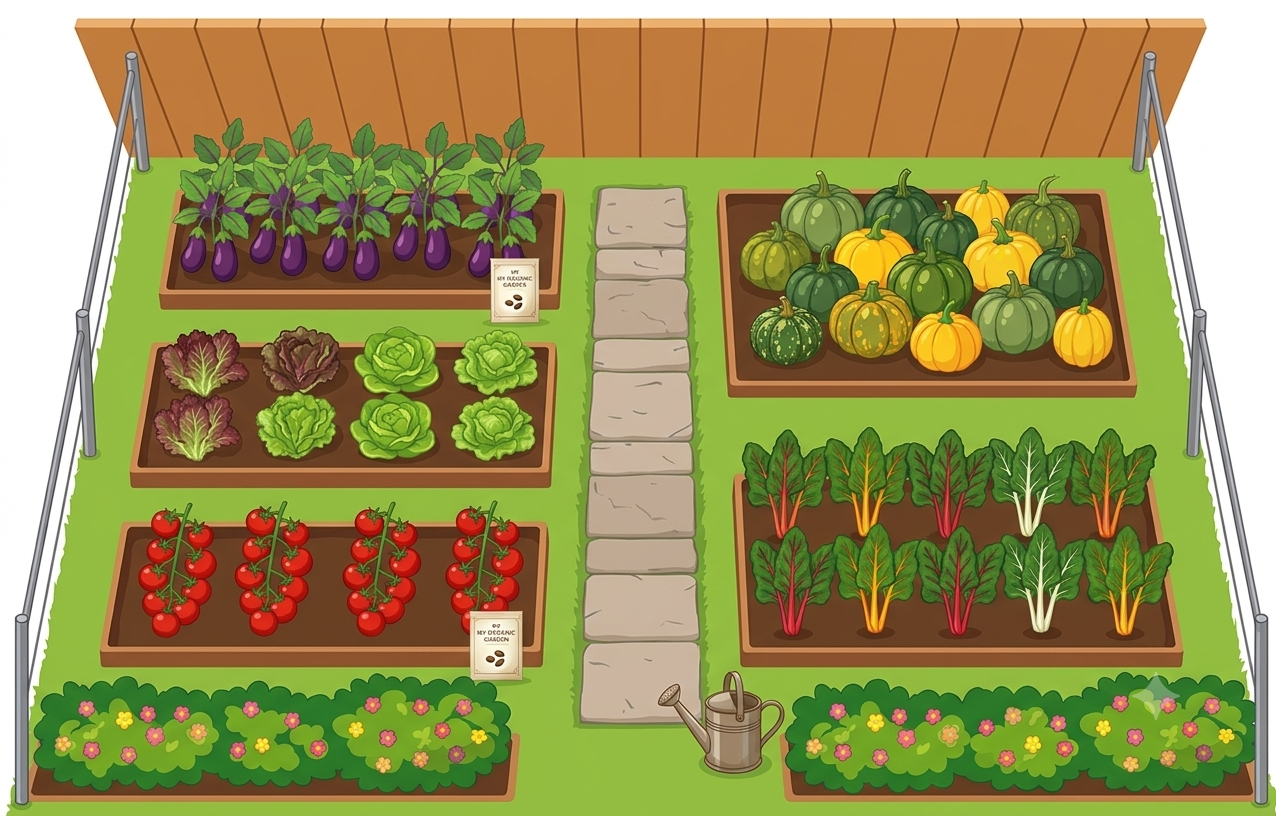
\includegraphics[width=5cm]{../images/NongTrai.png}
        };
    \end{scope}
\end{tikzpicture}
\end{center}}

% --- CÂU 24 ---
\questionShortAnswer{0}{24}{Một người nông dân có 18 000 000 đồng để làm một hàng rào hình chữ \( E \) dọc theo một con sông bao quanh hai khu đất trồng rau có dạng hai hình chữ nhật bằng nhau (hình vẽ). Đối với mặt hàng rào song song với bờ sông thì chi phí nguyên vật liệu là 60 000 đồng/mét, còn đối với ba mặt hàng rào song song nhau thì chi phí nguyên vật liệu là 20 000 đồng/mét, mặt giáp với bờ sông không phải rào. Tìm diện tích lớn nhất của hai khu đất thu được sau khi làm hàng rào (đơn vị: ha).

\begin{center}
\begin{tikzpicture}[>=latex, scale=0.8]
    \begin{scope}[xshift=0cm, yshift=0cm]
        \node[anchor=south west, inner sep=0] at (0,0) {
            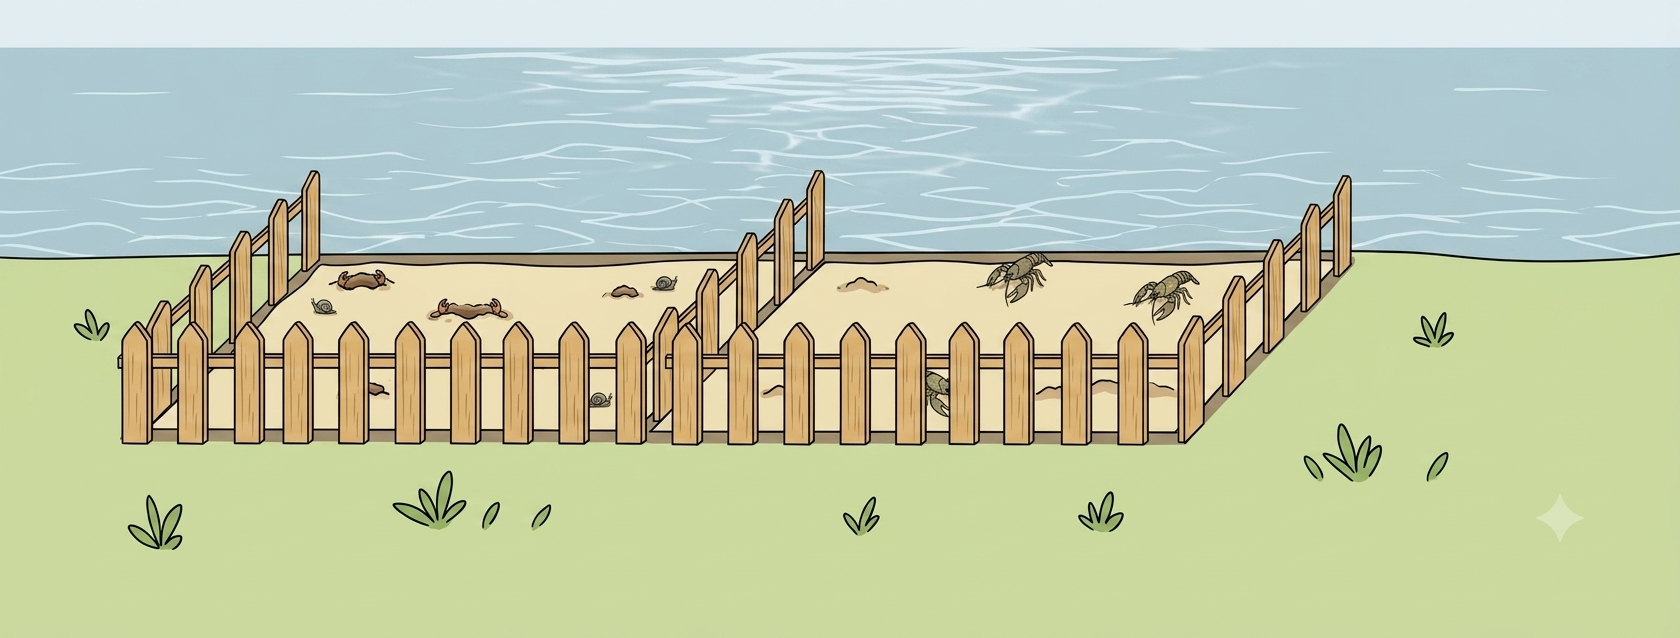
\includegraphics[width=5cm]{../images/HangRao.png}
        };
    \end{scope}
\end{tikzpicture}
\end{center}}

% --- CÂU 25 ---
\questionShortAnswer{0}{25}{Bạn Giang có một tấm tôn hình chữ nhật có chu vi 150cm. Bạn Giang muốn uốn tấm tôn trên thành một hình trụ (tham khảo hình vẽ). Biết rằng bạn Giang muốn hình trụ sau khi uốn có thể tích lớn nhất. Hỏi bạn Giang nên chọn tấm tôn hình chữ nhật có chiều dài là bao nhiêu cm?

\begin{center}
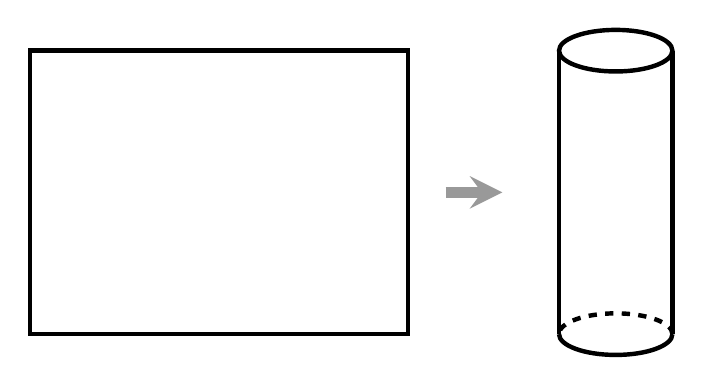
\begin{tikzpicture}[>=stealth, scale=1.2]

    % =================================================================
    % HÌNH BÊN TRÁI: HÌNH CHỮ NHẬT PHẲNG
    % =================================================================
    \begin{scope}[xshift=0cm, yshift=0cm]
        \draw[ultra thick] (0,0) rectangle (4,3);
    \end{scope}

    % Mũi tên chuyển bước ở giữa
    \draw[->, line width=4pt, gray!80] (4.4,1.5) -- (5.0,1.5);

    % =================================================================
    % HÌNH BÊN PHẢI: HÌNH TRỤ TRÒN (ĐÃ SỬA LỖI MẤT ĐỈNH)
    % =================================================================
    \begin{scope}[xshift=6.2cm, yshift=0cm]
        \def\R{0.6}    % Bán kính đáy elip 
        \def\H{3.0}    % Chiều cao hình trụ

        % Đáy trên: Vẽ toàn bộ bằng nét liền ôm sát hai cạnh bên
        \draw[ultra thick] (0,\H) ellipse [x radius=\R, y radius=0.22];

        % Đáy dưới: Nửa elip phía trước nét liền, nửa phía sau nét đứt
        \draw[ultra thick] (-\R,0) arc (180:360:\R\space and 0.22);
        \draw[ultra thick, dashed] (\R,0) arc (0:180:\R\space and 0.22);

        % Hai đường sinh đứng hai bên nối liền từ đáy lên đỉnh
        \draw[ultra thick] (-\R,0) -- (-\R,\H);
        \draw[ultra thick] (\R,0) -- (\R,\H);
    \end{scope}

\end{tikzpicture}
\end{center}}

% --- CÂU 26 ---
\questionShortAnswer{0}{26}{Công ty mĩ phẩm chuẩn bị cho ra một mẫu sản phẩm dưỡng da mới mang tên Ngọc Trai với thiết kế là một khối cầu như viên ngọc trai không lõi, bên trong là một khối trụ nằm trong khối cầu để đựng kem dưỡng da như hình vẽ. Nhà sản xuất dự định thiết kế khối cầu có bán kính là \( R = 4\sqrt{3} \, \text{cm} \). Tìm thể tích lớn nhất của khối trụ đựng kem (đơn vị: \( \text{cm}^3 \), kết quả làm tròn đến hàng đơn vị).

\begin{center}
\begin{tikzpicture}[>=latex, scale=0.5]
    \begin{scope}[xshift=0cm, yshift=0cm]
        \node[anchor=south west, inner sep=0] at (0,0) {
            
\includegraphics[width=3cm]{../images/DuongDa.png}
        };
    \end{scope}
\end{tikzpicture}
\end{center}}

% --- CÂU 27 ---
\questionShortAnswer{0}{27}{Một máng nước mưa được làm từ một tấm tôn rộng 45 cm bằng cách gấp hai phía của tấm tôn với kích thước bằng \(\dfrac{1}{3}\) tấm tôn sao cho nó tạo thành một góc \(x\) (như hình vẽ). Hỏi phải chọn \(x\) bằng bao nhiêu độ để máng chứa được lượng nước mưa tối đa.

\begin{center}
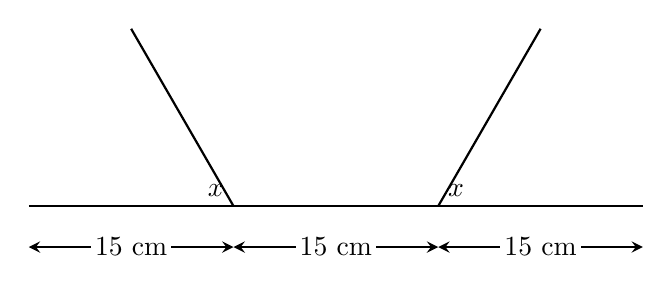
\begin{tikzpicture}[>=stealth, scale=1.3]

    % =================================================================
    % 1. VẼ ĐƯỜNG THẲNG NẰM NGANG VÀ CÁC ĐƯỜNG XIÊN
    % =================================================================
    % Đường thẳng nền nằm ngang dài 6 units
    \draw[thick] (0,0) -- (6,0);

    % Đường xiên bên trái (từ điểm x=2.0 đi lên sang trái, góc khoảng 120 độ)
    \draw[thick] (2.0,0) -- (1.0,1.732);

    % Đường xiên bên phải (từ điểm x=4.0 đi lên sang phải, góc khoảng 60 độ)
    \draw[thick] (4.0,0) -- (5.0,1.732);

    % =================================================================
    % 2. ĐIỀN CÁC KÝ HIỆU GÓC x
    % =================================================================
    % Góc x bên trái
    \node[above left] at (2.0,0) {$x$};
    
    % Góc x bên phải
    \node[above right] at (4.0,0) {$x$};

    % =================================================================
    % 3. VẼ HỆ THỐNG MŨI TÊN KÍCH THƯỚC PHÍA DƯỚI
    % =================================================================
    % Đoạn 15 cm bên trái
    \draw[<->, thick] (0,-0.4) -- (2.0,-0.4);
    \node[fill=white, inner sep=1.5pt] at (1.0,-0.4) {$15\text{ cm}$};

    % Đoạn 15 cm ở giữa
    \draw[<->, thick] (2.0,-0.4) -- (4.0,-0.4);
    \node[fill=white, inner sep=1.5pt] at (3.0,-0.4) {$15\text{ cm}$};

    % Đoạn 15 cm bên phải
    \draw[<->, thick] (4.0,-0.4) -- (6.0,-0.4);
    \node[fill=white, inner sep=1.5pt] at (5.0,-0.4) {$15\text{ cm}$};

\end{tikzpicture}
\end{center}}


\end{document}